\chapter[Exploration Round 4 - HyparHut]{Exploration Round 4\\HyparHut}
\label{chapter:exploration-round-4}

\section{Goal}
\label{section:exploration-4-goal}

The main goal of the fourth round is to address the accuracy, stability and alignment problems observed in the previous round, especially through the use of structural triangulation. Triangulation is a strategy commonly used in timber structural design for improving stiffness in the completed structure. However, this thesis will focus on improving the stiffness of the partially assembled (PA) structure during the assembly process. 

\todo{Added more description about the screw tool. This makes the entry to the first few sub-sections of 7.3 a bit easier.}
In addition, a new Screwdriver DiRT tool is developed to address the joint loosening problem \seeref{subsection:exploration-2-joints-loosening-after-assembly}, to assemble Non-Planar (NP) lap joints with flexible angles, and to assemble beams with different section sizes. The screwdriver mechanism is significantly different from the clamps used in previous rounds -- it assembles joints by rotating a long screw to pull the two halves of a joint together. In order to achieve these goals, the following development was performed:

\begin{itemize}
    \item \textbf{Mechatronics}
    \begin{itemize}
        \item \textbf{Screw Design --} a screw capable of pulling two joints together and leaving the screw behind \seeref{subsection:exploration-4-screw-design}
        \item \textbf{Screw Driving Mechanism --} a new operation principle for driving the screw into the joint \seeref{subsection:exploration-4-screw-driving-mechanism}
        \item \textbf{Screwdriver Hardware --} a integrated solution of the screw driving mechanism and a gripper for it to hand onto the beam \seeref{subsection:exploration-4-lap-screwdriver-sl1-and-sl1-g200-hardware}
        \item \textbf{Ground Platform Design --} an improved connection for the initial elements to the foundation platform \seeref{subsection:exploration-4-beam-to-ground-connection}
    \end{itemize}
    \item \textbf{Design Guideline}
    \begin{itemize}
        \item Deformation-aware design approach \seeref{subsection:exploration-4-deformation-awareness-and-error-correction-by-triangulation}
    \end{itemize}
    \item \textbf{CAD Modeling}
    \begin{itemize}
        \item Parametric Polyline Lap Joints \seeref{subsection:exploration-4-parametric-polyline-lap-joints}
    \end{itemize}
    \begin{itemize}
        \item Parametric Non-Planar Lap Joints\seeref{subsection:exploration-4-parametric-non-planar-lap-joints}
    \end{itemize}
    \item \textbf{CAM Modeling}
    \begin{itemize}
        \item Flying Screwdriver Movements\seeref{subsection:exploration-4-process-design-interface-for-screw-assembly-process}
    \end{itemize}
\end{itemize}

\subsection{Deformation-Awareness and Error Correction by Triangulation}
\label{subsection:exploration-4-deformation-awareness-and-error-correction-by-triangulation}

This is a new framework developed from the observation in previous experiments \seeref{subsection:exploration-2-corrective-effects-of-adding-elements}. The observation provided an indication that the addition of more elements helped correct the deformation in the partial structure. This effect was present as long as there were more than one joint being assembled, and the effect is more pronounced when a new triangle is formed. 

\paragraph{Hypothesis}

I propose the hypothesis that the source of deformation originates from the low stiffness of the lap joints, and that it is possible to approximate the structural behaviour joints behave like a kinematic hinge. Therefore, the addition of a constraining element will add new kinematic constraints to the system. If the system becomes fully constrained, for example by creating triangles, a rigid and stable frame can be formed.

When adding a new element to constrain a frame, if deformation is present in the already-assembled structure, it is by definition not possible to perfectly align the joints between the new element and the existing structure. However, thanks to the chamfer guidance mechanism, perfect alignment is not necessary to begin the assembly.

During the joint closure, the guidance offered by the chamfer will push the joints against each other to force them into agreement. Because the joints on the robot-side all belong to the same beam, these joints are very stiff. On the stationary-side, the joints are located on different beams of the Partially Assembled (PA) structure. Therefore, their positions are much more susceptible to being moved by the DiRT tool's assembly force. 

Note that the corrective force is provided by the DiRT tool force that is redirected by the chamfering angle. The angle of the chamfer and its contact friction determines how much force will be redirected. The success of this correction will therefore be determined by the design of the chamfer geometry and the maximum force that can be provided by the DiRT tools. 

Additionally the correctness that can be achieved by this method, relies on the accuracy of the machined joints. Specifically, the location between the joints will be crucial to ensure that the rigid triangles are of the same shape. The tightness of the joint will also affect the residual deformation in the system, because any looseness introduces extra unconstrained freedom to the kinematic system. 

\paragraph{Validation}
The implementation of the principle above will consist of two steps. The first is to identify the high risk elements that are prone to deformation and are likely to cause an alignment failure in the subsequent assembly process. The second step is to modify the structure, or to change the assembly sequence to mitigate the problem.

Both of the tasks are loosely defined at this stage because it is not clear what constitutes high deformation risk and what is the appropriate correction strategy. However, I speculate that the following properties can indicate a high risk element:
\begin{itemize}
    \item Long elements with long unsupported portions
    \item Elements with only one joint
    \item Highly unbalanced or cantilevering elements
\end{itemize}

Note that it is important to consider how the element can deform, and predict the deviation at the location where the next alignment is needed. Figure \ref{fig:deviation-on-column-depends-on-location} shows a column that is only fixed by one joint, this is a high risk element because the joint can rotate left or right. If the next joint to be assembled is near the existing joint (\ref{fig:deviation-on-column-depends-on-location}b), the amount of deviation will be less than if the joint is far away (\ref{fig:deviation-on-column-depends-on-location}c). 

\begin{figure}[!h]
    \centering
    \includegraphics[width=0.99\textwidth]{images/7a/img01.jpg}
    \caption[Diagram showing the deviation on a column depends on the location of the next joint]
    {Diagram showing the deviation on a column depends on the location of the next joint. The deviation is less when the next joint is near and more when the next joint is far away.}
    \label{fig:deviation-on-column-depends-on-location}
\end{figure}

In general, the correction goal is to minimise the risk of alignment error. This can include:
\begin{itemize}
    \item Changing assembly sequence
    \item Changing position of the beam arrangements
    \item Adding diagonal bracing to introduce triangles
\end{itemize}

The details of how this is applied to the demonstrator in this round can be found in a later section \seeref{subsubsection:exploration-4-global-correction-approach}.

\section{Background}
\label{section:exploration-4-background}

\subsection{Machining Limitation for cutting Lap Joints}
\label{subsection:exploration-4-cnc-limitation-in-cutting-lap-joints}

There is a wide variety of automatic joinery machines in the market. Depending on the kinematics of the spindle and the tools that it has, it can produce different types of joints. There are three main types of cutting tools used in an automatic joinery machine, saws, planar mills and end mills (see Figure \ref{fig:tools-in-automatic-joinery-machine}). 


% 2 Horizontal Image  
\begin{figure}[!h]
    \centering
    \begin{subfigure}[b]{0.49\textwidth}
        \centering
        \includegraphics[width=\textwidth]{images/7a/img02.jpg}
        \caption{Planar Mill in operation}
        %\label{fig:uniquesubfigurelabel}
    \end{subfigure}
    \hfill
    \begin{subfigure}[b]{0.49\textwidth}
        \centering
        \includegraphics[width=\textwidth]{images/7a/img03.jpg}
        \caption{Typical Tool Storage}
        %\label{fig:uniquesubfigurelabel}
    \end{subfigure}
    \caption[Different tools in a automatic joinery machine]
    {Different tools in a automatic joinery machine.
    \footnotesize{(Credits: Photos by Hans Hundegger AG, retrieved from https://www.hundegger.com/maschinen/abbundmaschinen/k2-industry, 2020)}}
    \label{fig:tools-in-automatic-joinery-machine}
\end{figure}


Depending on the joint type, angles and sizes, different tools are selected for the cutting task. In many cases, there is a default tool for a certain type of joint. However, there are also cases where a joint can be created with different types of tools. For example, a bird's mouth joint, a 90 degrees notch cut-out on the edge of a beam, can be milled with a planar mill (turning all the material into sawdust) or it can be cut with two saw cuts (cutting out the offcut piece).

Many of the cutting tools used by an automatic joinery machine (image above, left and right) have a cylindrical profile with a flat end. This geometry is imparted on the timber material as the cutter moves along the wood. Even a saw blade has its thickness, and the front side can be seen as a right-angle face to its sides. Therefore the most acute angle that can be created with these tools is a right angle.\footnote{The exception to this is to use a profile cutter that does not have a cylindrical cutting shape. Such as a dovetail cutter or a conical end mill. However, they are not suitable for creating lap joints.}

When cutting a lap joint, the planar mill is the most common tool choice (image above, left). Therefore, when designing a complex lap joint \seerefii{subsection:exploration-4-parametric-polyline-lap-joints}{subsection:exploration-4-parametric-non-planar-lap-joints}, it is important to avoid creating interior corners that are less than 90 degrees. In addition, it is necessary to ensure that the flat area inside the lap joint (a.k.a. The trench that is left over from the mill) is at least as wide as the planar mill’s width and the depth of the cut can be made by the cutter.

Figure \ref{fig:non-planar-lap-joint-with-compound-angles} shows a non planar lap joint with compound angles. The cut-away path of the planar mill is visualised by the green and cyan rectangular boxes (Figure \ref{fig:cut-away-path-of-the-planar-mill}). The 25mm indicated in the drawing referred to an hypothetical width of a planar mill, in this case, four parallel passes would be needed to create one of the 100mm faces. The 80mm indicated in the drawing refers to the maximum depth of the cutter. Joints that are deeper than this cut are still possible, but will have to use an end mill instead of a planar mill.


% 2 Horizontal Image  
\begin{figure}[!h]
    \centering
    \begin{subfigure}[b]{0.49\textwidth}
        \centering
        \includegraphics[width=\textwidth]{images/7a/img04.jpg}
        \caption{Non-planar lap joint with compound angles}
        \label{fig:non-planar-lap-joint-with-compound-angles}
    \end{subfigure}
    \hfill
    \begin{subfigure}[b]{0.49\textwidth}
        \centering
        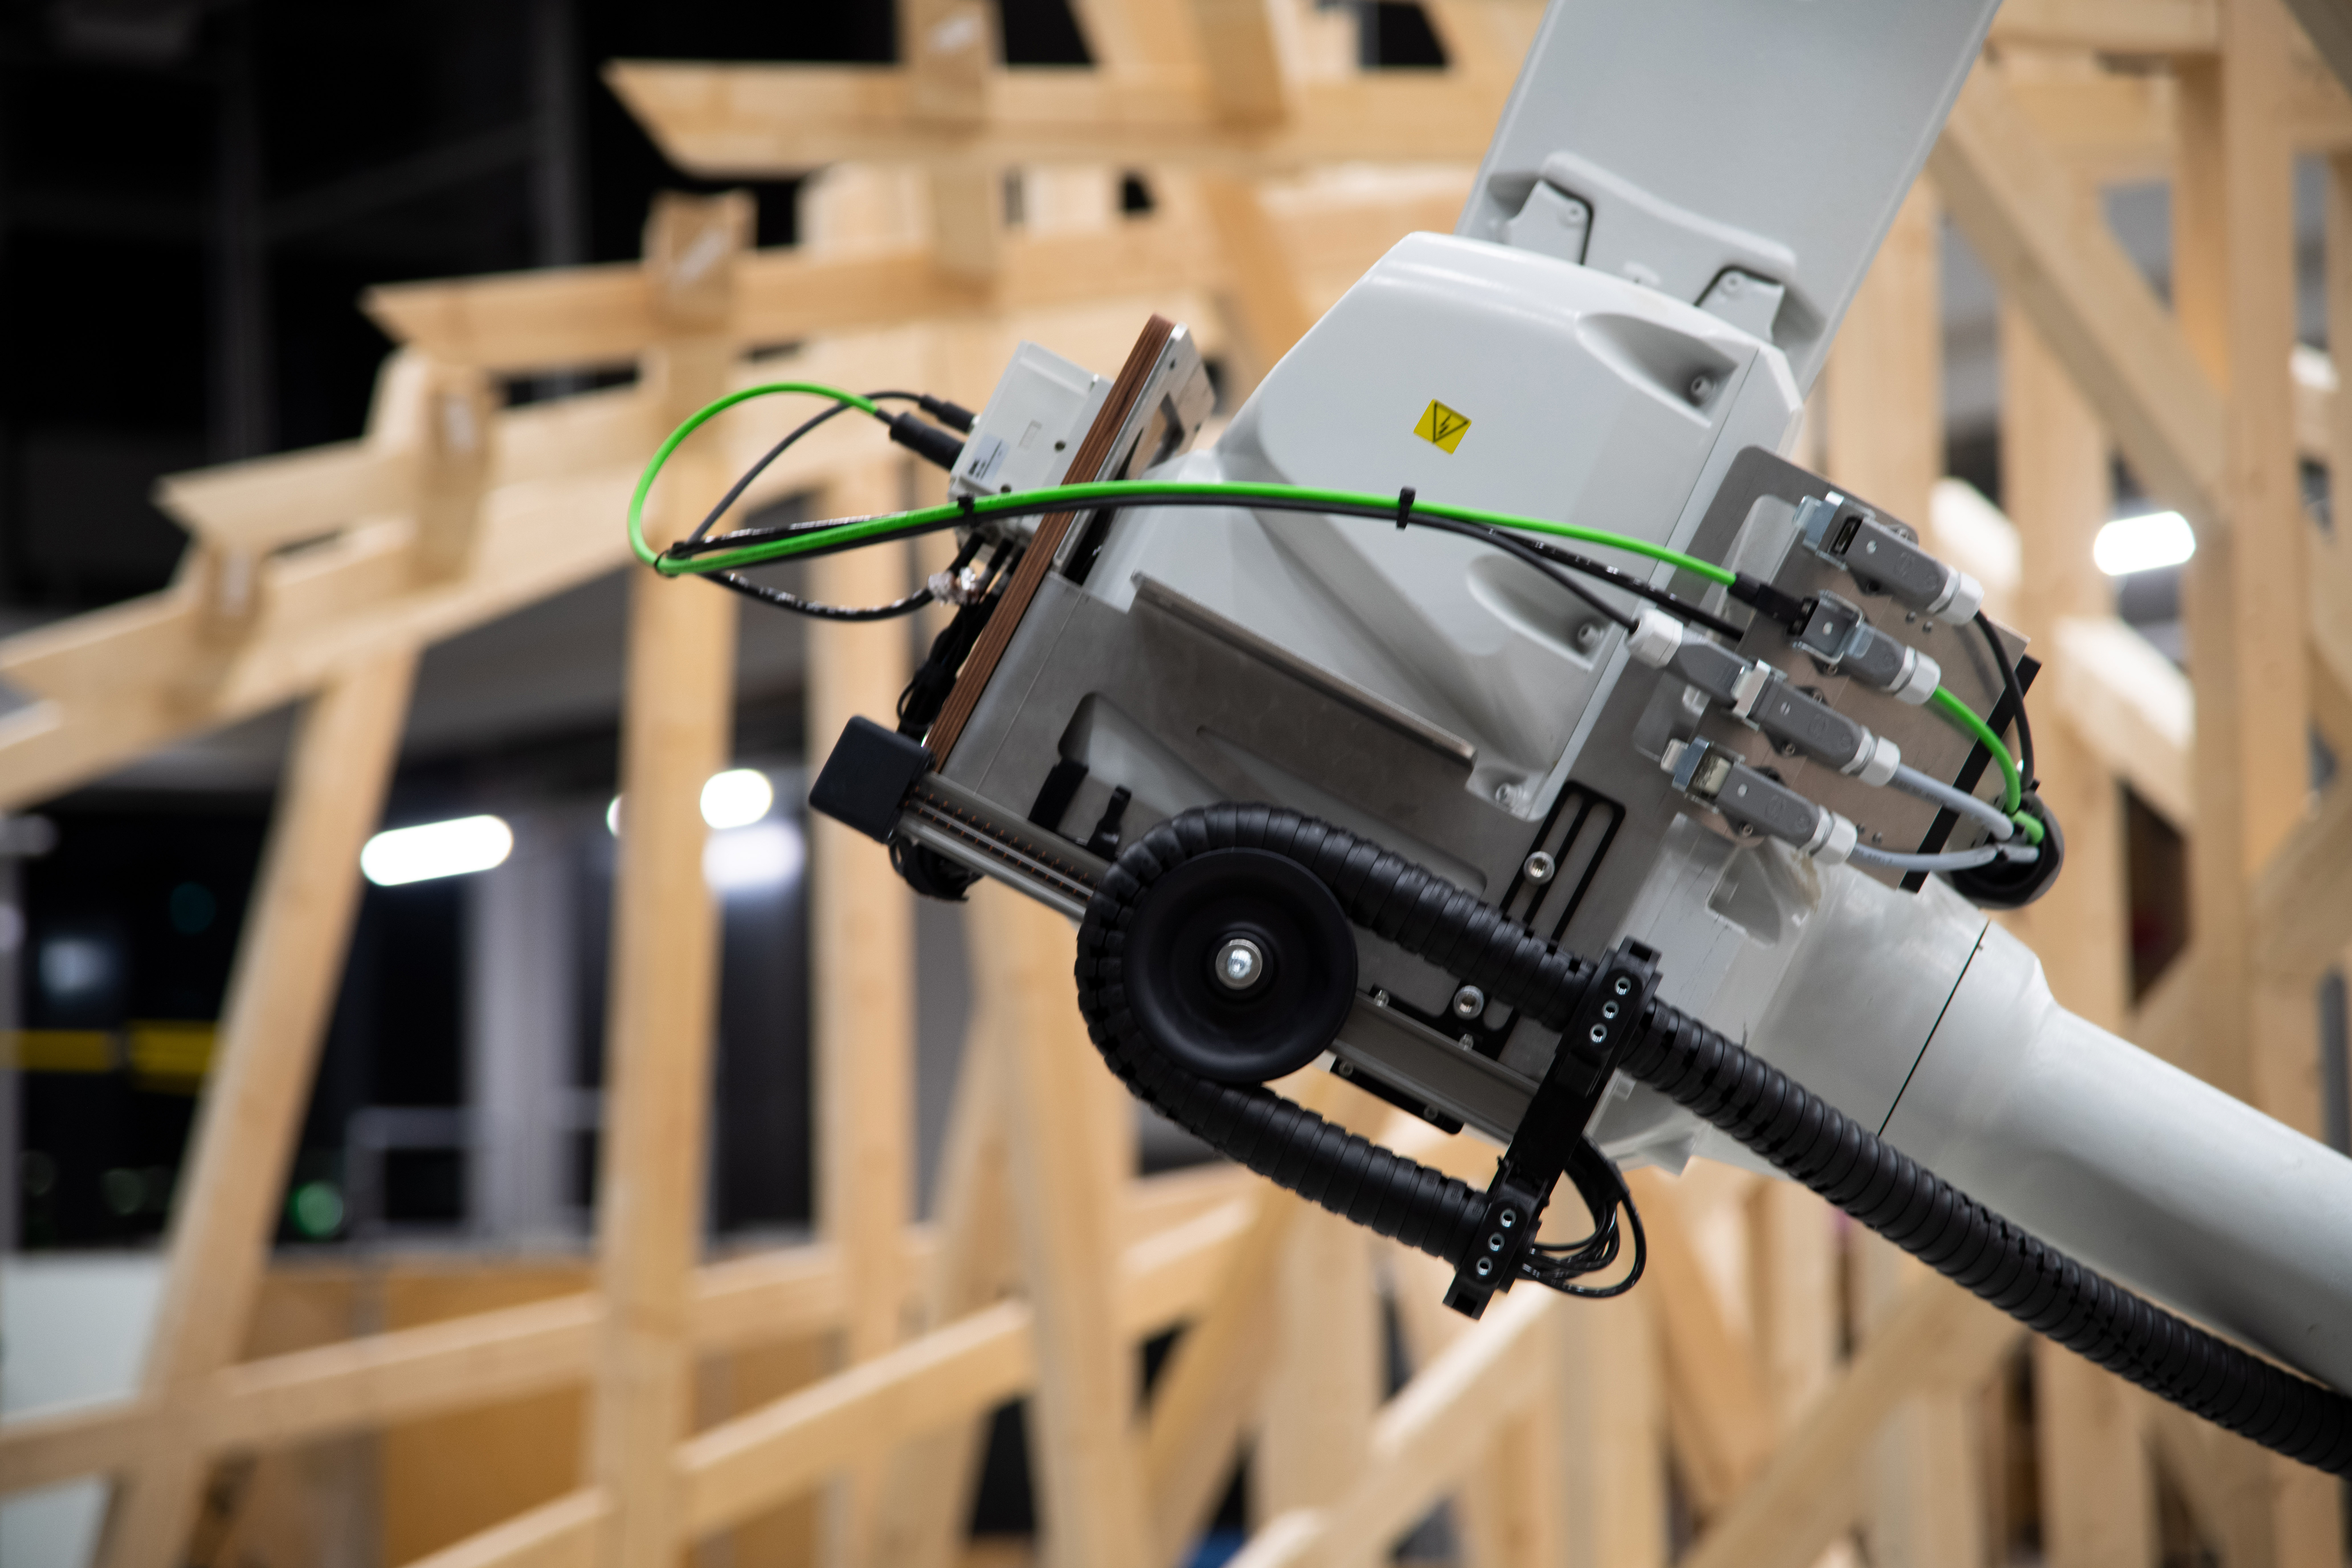
\includegraphics[width=\textwidth]{images/7a/img05.jpg}
        \caption{Cut-away path of the planar mill}
        \label{fig:cut-away-path-of-the-planar-mill}
    \end{subfigure}
    \caption{Digital model of a non-planar lap joint with compound angles}
    \label{fig:model-non-planar-lap-joint}
\end{figure}


Figure \ref{fig:angle-checking-routine} shows a generalised checking routine for the joint geometry that ensures no interior acute angles. This check is performed after design time to ensure that the joints are parametrized correctly. Problematic geometries that are passed to the fabricator will also be flagged by their CAM software, in addition to many other machine limitations that may prevent a joint from being fabricated. However, a checking routine that is closer to design time allows a faster feedback for the designer.


% 2 Horizontal Image  
\begin{figure}[!h]
    \centering
    \begin{subfigure}[b]{0.49\textwidth}
        \centering
        \includegraphics[width=\textwidth]{images/7a/img06.jpg}
        % \caption{SubFigureCaption}
        %\label{fig:uniquesubfigurelabel}
    \end{subfigure}
    \hfill
    \begin{subfigure}[b]{0.49\textwidth}
        \centering
        \includegraphics[width=\textwidth]{images/7a/img07.jpg}
        % \caption{SubFigureCaption}
        %\label{fig:uniquesubfigurelabel}
    \end{subfigure}
    \caption{Angle checking routine for ensuring no interior acute angles}
    \label{fig:angle-checking-routine}
\end{figure}


\section{Development}
\label{section:exploration-4-development}

\subsection{Parametric Polyline Lap Joints}
\label{subsection:exploration-4-parametric-polyline-lap-joints}

The polyline lap joint is an extended version of the simple lap joint that was used in the previous round. The intention is to create a parametric model that is able to include historical lap joint designs.

The model consists of four polylines that are used to describe the geometry on each of the four shoulders of the lap joint. Each polyline consists of at least one straight segment to describe the face. The polyline points are defined as parametric 2D points in reference to the intersection quad of the two beams. The exact shape of the polyline will, therefore, depend on the width of the two beams, and it can morph (stretch) automatically onto any intersection. Figure \ref{fig:polyine-lap-joint-adaptability} and \ref{fig:polyine-lap-joint-adaptability-2} show the adaptability of the polyline being used to encode different joint designs.

\begin{figure}[!h]
    \centering
    \includegraphics[width=0.99\textwidth]{images/7a/img08.jpg}
    \caption{Diagram showing the adaptability of the polyline lap joint being used to encode a bowtie joint}
    \label{fig:polyine-lap-joint-adaptability}
\end{figure}

% 3 x 2 Images
\begin{figure}[!h]
    \centering
    \begin{subfigure}[b]{0.49\textwidth}
        \centering
        \includegraphics[width=\textwidth]{images/7a/img09.jpg}
        % \caption{SubFigureCaption}
        %\label{fig:uniquesubfigurelabel}
    \end{subfigure}
    \hfill
    \begin{subfigure}[b]{0.49\textwidth}
        \centering
        \includegraphics[width=\textwidth]{images/7a/img10.jpg}
        % \caption{SubFigureCaption}
        %\label{fig:uniquesubfigurelabel}
    \end{subfigure}
    \vskip\baselineskip % Next row
    \begin{subfigure}[b]{0.49\textwidth}
        \centering
        \includegraphics[width=\textwidth]{images/7a/img11.jpg}
        % \caption{SubFigureCaption}
        %\label{fig:uniquesubfigurelabel}
    \end{subfigure}
    \hfill
    \begin{subfigure}[b]{0.49\textwidth}
        \centering
        \includegraphics[width=\textwidth]{images/7a/img12.jpg}
        % \caption{SubFigureCaption}
        %\label{fig:uniquesubfigurelabel}
    \end{subfigure}
    \vskip\baselineskip % Next row
    \begin{subfigure}[b]{0.49\textwidth}
        \centering
        \includegraphics[width=\textwidth]{images/7a/img13.jpg}
        % \caption{SubFigureCaption}
        %\label{fig:uniquesubfigurelabel}
    \end{subfigure}
    \hfill
    \begin{subfigure}[b]{0.49\textwidth}
        \centering
        \includegraphics[width=\textwidth]{images/7a/img14.jpg}
        % \caption{SubFigureCaption}
        %\label{fig:uniquesubfigurelabel}
    \end{subfigure}
    \caption{Diagram showing the polyline lap joint adapting into different joint designs}
    \label{fig:polyine-lap-joint-adaptability-2}
\end{figure}

Because of the morph, there is no inherent protection against modelling a joint that cannot be machined. However, a simple machinability check can be performed after the morph by measuring the angles at the polyline kinks. There are no automatic solutions included to make the joint machinable. Figure \ref{fig:non-machinable-details-in-a-joint} shows the same polyline definition morphed into different intersection angles. Figure \ref{fig:joint-not-machinable} is machinable because all machining angles are larger than 90 degrees. Figure \ref{fig:joint-machinable} is not machinable because one of the angles is less than 90 degrees. \seeref{subsection:exploration-4-cnc-limitation-in-cutting-lap-joints}

% 2 Horizontal Image  
\begin{figure}[!h]
    \centering
    \begin{subfigure}[b]{0.49\textwidth}
        \centering
        \includegraphics[width=\textwidth]{images/7a/img15.jpg}
        \caption{Machinable}
        \label{fig:joint-machinable}
    \end{subfigure}
    \hfill
    \begin{subfigure}[b]{0.49\textwidth}
        \centering
        \includegraphics[width=\textwidth]{images/7a/img16.jpg}
        \caption{Not Machinable}
        \label{fig:joint-not-machinable}
    \end{subfigure}
    \caption{Diagram showing non-machinable details in a joint after it morphed into different intersection angles}
    \label{fig:non-machinable-details-in-a-joint}
\end{figure}

\FloatBarrier

\subsection{Parametric Non-Planar Lap Joints}
\label{subsection:exploration-4-parametric-non-planar-lap-joints}

The non-planar lap joint was created to model the non-planar intersection of two beams forming a lap joint. The model is able to adapt to all three types of intersection angles (planar angle, out-of-plane angle, and axial angle). The joint has a fixed assembly direction that is perpendicular to the beam that is moving with the robot (in the diagrams below, the top side of the beam is the moving beam). The assembly direction also equates to the axis of the attached screwdriver because that is the only possible way it can assemble the joint.

The parametric model was designed to automatically keep the face-to-face angles to at least 90 degrees, thereby ensuring machinability automatically. However, it is necessary to adjust the depth of the cheek manually to ensure that the joint has enough material on either side to be structurally strong.

Figure \ref{fig:difference-out-of-plane-angle} below show the difference between a joint having only a planar angle (\ref{fig:only-planar-angle}) and when an out-of-plane angle is added to it (\ref{fig:and-out-of-plane-angle}).

% 2 Horizontal Image  
\begin{figure}[!h]
    \centering
    \begin{subfigure}[b]{0.49\textwidth}
        \centering
        \includegraphics[width=\textwidth]{images/7a/img17.jpg}
        \caption{Only planar angle}
        \label{fig:only-planar-angle}
    \end{subfigure}
    \hfill
    \begin{subfigure}[b]{0.49\textwidth}
        \centering
        \includegraphics[width=\textwidth]{images/7a/img18.jpg}
        \caption{Planar angle and out-of-plane angle}
        \label{fig:and-out-of-plane-angle}
    \end{subfigure}
    \caption{Diagram showing the difference between a joint having only a planar angle and with out-of-plane angle}
    \label{fig:difference-out-of-plane-angle}
\end{figure}

Figure \ref{fig:axial-angle} below shows the same joint with planar angle and out-of-plane angle, before (\ref{fig:no-axial-angle-yet}) and after axial angle is added to it (\ref{fig:axial-angle-added}). Notice that when axial angle is added to it, one of the parallel faces will no longer be parallel. 

% 2 Horizontal Image  
\begin{figure}[!h]
    \centering
    \begin{subfigure}[b]{0.49\textwidth}
        \centering
        \includegraphics[width=\textwidth]{images/7a/img19.jpg}
        \caption{Planar angle and out-of-plane angle}
        \label{fig:no-axial-angle-yet}
    \end{subfigure}
    \hfill
    \begin{subfigure}[b]{0.49\textwidth}
        \centering
        \includegraphics[width=\textwidth]{images/7a/img20.jpg}
        \caption{Planar angle, out-of-plane angle and axial angle}
        \label{fig:axial-angle-added}
    \end{subfigure}
    \caption{Diagram showing the addition of axial angle to a joint with planar angle and out-of-plane angle}
    \label{fig:axial-angle}
\end{figure}

The parametrization of the joint cannot accommodate a large intersection angle, this is inherent to the intersection area of the timber beams. Figure \ref{fig:large-out-of-plane-angle} shows a joint with a large out-of-plane angle, the intersection area is very large and the material that needs to be removed on either side of the beam will be significant. In the image, the lower beam has a lot of material removed, causing it to be a weak side. Figure \ref{fig:large-axial-angle} shows a joint with a large axial angle, it contains only a small amount of parallel walls. This will reduce the shear capacity and rotational stiffness of the joint.

% 2 Horizontal Image  
\begin{figure}[!h]
    \centering
    \begin{subfigure}[b]{0.49\textwidth}
        \centering
        \includegraphics[width=\textwidth]{images/7a/img21.jpg}
        \caption{Joint with large out-of-plane angle}
        \label{fig:large-out-of-plane-angle}
    \end{subfigure}
    \hfill
    \begin{subfigure}[b]{0.49\textwidth}
        \centering
        \includegraphics[width=\textwidth]{images/7a/img22.jpg}
        \caption{Joint with large axial angle}
        \label{fig:large-axial-angle}
    \end{subfigure}
    \caption{Diagram showing the limitation of the parametric non-planar lap joint}
    \label{fig:limitation-parametric-non-planar-lap-joint}
\end{figure}

The interaction of the three angles produces different joint results that have different amounts of overlap. When designing the demonstrator, it was possible to manually adjust the cheek depth to balance the two sides of a joint. However, automatic adjustment was not implemented. Figure \ref{fig:low-high-cheek-depth} shows the difference between a low and high cheek depth. 

% 2 Horizontal Image  
\begin{figure}[!h]
    \centering
    \begin{subfigure}[b]{0.49\textwidth}
        \centering
        \includegraphics[width=\textwidth]{images/7a/img23.jpg}
        \caption{Low Cheek Depth} 
        %\label{fig:uniquesubfigurelabel}
    \end{subfigure}
    \hfill
    \begin{subfigure}[b]{0.49\textwidth}
        \centering
        \includegraphics[width=\textwidth]{images/7a/img24.jpg}
        \caption{High Cheek Depth}
        % \label{fig:uniquesubfigurelabel}
    \end{subfigure}
    \caption{Diagram showing the difference between a low and high cheek depth}
    \label{fig:low-high-cheek-depth}
\end{figure}


\subsection{Screw Design}
\label{subsection:exploration-4-screw-design}

The design of the screw precedes the design of the screwdriver. The goal of the screw design consists of two parts. 

\begin{enumerate}
    \item The screw has to pull the two halves of the joints together.
    \item The screw has to stay behind to secure the joint against loosening \seeref{subsection:exploration-2-joints-loosening-after-assembly}.

\end{enumerate}
The two requirements have a conflicting requirement because the screw needs to be longer than the lap joint when it is not assembled for step 1, but has to be shorter than the total joint thickness after it is left behind, such that the screw does not stick outside of the timber. 

This conflict led to the design of a two-screw design where a long and thin screw is used to pull the joint, while another short and hollow screw is left behind after the assembly. Both screws have the same pitch so they can be tightened with the same rotation.

Figure \ref{fig:two-screw-design} shows the two screws placed on the moving side of the beam before they are assembled. The tip of the pull screw is about to engage with a predrilled hole on the stationary side of the beam.

\begin{figure}[!h]
    \centering
    \includegraphics[width=0.99\textwidth]{images/7a/img25.png}
    \caption{Diagram showing the two-screw design}
    \label{fig:two-screw-design}
\end{figure}

In the subsequent movement, the two screws will rotate together and move towards the stationary side of the joint. The receiving hole has two steps, the smaller of the two steps will engage with the pull screw and create the pulling force (Figure \ref{fig:two-screw-operation}, step 1). This pull force is the main assembly force used for closing the joint including the correction forces when the edge chamfers engage (Figure {fig:two-screw-operation}, step2).

As the motion continues, the left-in screw will engage with the receiving hole, it will be threaded to the larger step of the hole (Figure \ref{fig:two-screw-operation}, step 3). The screwing motion is continued until the joint is tightly assembled (Figure \ref{fig:two-screw-operation}, step 4). Afterwards, the centre screw will unscrew from the joint while the left-in screw will stay with the joint \seeref{subsection:exploration-4-screw-driving-mechanism}.

% 2 x 2 Images
\begin{figure}[!h]
    \centering
    \begin{subfigure}[b]{0.49\textwidth}
        \centering
        \includegraphics[width=\textwidth]{images/7a/img26.png}
        \caption*{Step 1}
        %\label{fig:uniquesubfigurelabel}
    \end{subfigure}
    \hfill
    \begin{subfigure}[b]{0.49\textwidth}
        \centering
        \includegraphics[width=\textwidth]{images/7a/img27.png}
        \caption*{Step 2}
        %\label{fig:uniquesubfigurelabel}
    \end{subfigure}
    \vskip\baselineskip % Next row
    \begin{subfigure}[b]{0.49\textwidth}
        \centering
        \includegraphics[width=\textwidth]{images/7a/img28.png}
        \caption*{Step 3}
        %\label{fig:uniquesubfigurelabel}
    \end{subfigure}
    \hfill
    \begin{subfigure}[b]{0.49\textwidth}
        \centering
        \includegraphics[width=\textwidth]{images/7a/img29.png}
        \caption*{Step 4}
        %\label{fig:uniquesubfigurelabel}
    \end{subfigure}
    \caption{Diagram showing the sequence of operation of the two-screw design}
    \label{fig:two-screw-operation}
\end{figure}

\FloatBarrier

The screws were tested empirically to determine the size of the threads and the predrilled hole (see Figure \ref{fig:hollow-screw-test}). The goal is to find a balance between tightening torque and holding force. One of the optimizations after testing is the addition of thread-cutting slots (\ref{fig:screw-samples-with-thread-cutting-slots}) on the side of the hollow screw, this lowers the tightening torque while ensuring a good holding force. 
The screw design and the screw prototypes are made by Luca Steiner (Luca Stephan Steiner, 2020) under the supervision of Prof. Dr. Agathe Koller-Hodac and Marco Rossi.

% 2 x 2 Images
\begin{figure}[!h]
    \centering
    \begin{subfigure}[b]{0.49\textwidth}
        \centering
        \includegraphics[width=\textwidth]{images/7a/img30.jpg}
        \caption{Screw samples with thread-cutting slots drilled from the side}
        \label{fig:screw-samples-with-thread-cutting-slots}
    \end{subfigure}
    \hfill
    \begin{subfigure}[b]{0.49\textwidth}
        \centering
        \includegraphics[width=\textwidth]{images/7a/img31.jpg}
        \caption{Testing setup for measuring the tightening force and holding force}
        %\label{fig:uniquesubfigurelabel}
    \end{subfigure}
    \vskip\baselineskip % Next row
    \begin{subfigure}[b]{0.49\textwidth}
        \centering
        \includegraphics[width=\textwidth]{images/7a/img32.jpg}
        \caption{Screw sample placed in a predrilled hole in a lap joint}
        %\label{fig:uniquesubfigurelabel}
    \end{subfigure}
    \hfill
    \begin{subfigure}[b]{0.49\textwidth}
        \centering
        \includegraphics[width=\textwidth]{images/7a/img33.jpg}
        \caption{Screws produced for the demonstrator with zinc plating for anti-corrosion} 
        %\label{fig:uniquesubfigurelabel}
    \end{subfigure}
    \caption{Photos of the testing articles of the hollow screw}
    \label{fig:hollow-screw-test}
\end{figure}

\subsection{Screw Driving Mechanism}
\label{subsection:exploration-4-screw-driving-mechanism}

The screw driving mechanism was designed to actuate the two-screw design \seeref{subsection:exploration-4-screw-design}. The goal of the mechanical movements consist of two tasks:

\begin{enumerate}
    \item \textbf{Pull together two joint halves} by rotating the pull screw and the hollow screw. The screwdriver moves together with the moving beam towards the stationary-side.
    \item \textbf{Unscrew the pull screw} The screwdriver moves backward while both beams and the hollow screw stay stationary.
\end{enumerate}

The main concept of the driving mechanism is the single-direction screw driving head, which consists of a freewheel clutch.\footnote{A freewheel clutch is a circular bearing that allow the transmission of torque only in one direction. During transmission, the driving side and the outside of the bearing is locked together. If the driving side reverse in direction, the output side will be unlocked and does not receive torque.} This allows the use of only a single motor to actuate both screws. The motor is connected to the centre pull screw through a worm gearbox. During the CW rotation motion in step one, the rotation of the centre screw is transferred to the hollow screw drive hub through the freewheel clutch. Therefore both screws are tightened at the same time. During the CCW rotation of step two, only the centre pull screw is rotated. Therefore the hollow screw will be left behind as the centre screw retracts.

Figure \ref{fig:luca-prototype} shows the first prototype of the screw-driving mechanism, Figure \ref{fig:later-prototype} shows the next iteration that included the worm gearbox. 

% 2 Horizontal Image  
\begin{figure}[!h]
    \centering
    \begin{subfigure}[b]{0.49\textwidth}
        \centering
        \includegraphics[width=\textwidth]{images/7a/img34.jpg}
        \caption{Early prototype by Luca Stephan Steiner}
        \label{fig:luca-prototype}
    \end{subfigure}
    \hfill
    \begin{subfigure}[b]{0.49\textwidth}
        \centering
        \includegraphics[width=\textwidth]{images/7a/img35.jpg}
        \caption{Later prototype integrated with worm drive gearbox}
        \label{fig:later-prototype}
    \end{subfigure}
    \caption{Photos of the screw driving mechanism prototypes}
    \label{fig:photos-of-the-screw-driving-mechanism-prototypes}
\end{figure}

Learning from the stalling experience from the CL3 clamp, the selection of the main motor was conservative and with a higher safety factor. During the construction of the demonstrator, the screwdriver never stalled because of insufficient torque. Figure \ref{fig:motors-that-were-tested} shows different motors that were tested. Figure \ref{fig:construction-of-the-screw-driving-head} shows the construction of the screw-driving head. The free wheel clutch and the front bearing can be seen. Two cylindrical magnets were mounted on the driver head for retaining the hollow screw.
Figure \ref{fig:keyway-interface} shows the detail of the centre pull screw, the keyway can be seen that transfer torque between the worm gearbox and the freewheel clutch. Figure \ref{fig:pull-screw-head-assembled} shows the freewheel clutch and the driver head installed.

% 2 Horizontal Image  
\begin{figure}[!h]
    \centering
    \begin{minipage}{0.49\textwidth}
        \centering
        \includegraphics[width=\textwidth]{images/7a/img36.jpg}
        \caption{Motors that were tested for the screwdriver}
        \label{fig:motors-that-were-tested}
    \end{minipage}
    \hfill
    \begin{minipage}{0.49\textwidth}
        \centering
        \includegraphics[width=\textwidth]{images/7a/img37.jpg}
        \caption{Construction of the screw-driving head with freewheel clutch and front bearing}
        \label{fig:construction-of-the-screw-driving-head}
    \end{minipage}
    % \caption{FigureCaption}
    %\label{fig:uniquefigurelabel}
\end{figure}

\begin{figure}[!h]
    \centering
    \begin{minipage}{0.49\textwidth}
        \centering
        \includegraphics[width=\textwidth]{images/7a/img38.jpg}
        \caption{The pullscrew connects between the gearbox and the freewheel clutch}
        \label{fig:keyway-interface}
    \end{minipage}
    \hfill
    \begin{minipage}{0.49\textwidth}
        \centering
        \includegraphics[width=\textwidth]{images/7a/img39.jpg}
        \caption{Pull screw and the screw driver head assembled}
        \label{fig:pull-screw-head-assembled}
    \end{minipage}
    % \caption{FigureCaption}
    %\label{fig:uniquefigurelabel}
\end{figure}

\FloatBarrier

\subsection{Pin Gripper Mechanism}
\label{subsection:exploration-4-pin-gripper-mechanism}

The pin gripper mechanism is developed for attaching the robotic screwdriver to the beam. The motivation is to avoid the limitation of parallel grippers, where the jaws need to open towards the two sides and limit beams from being placed next to each other. 

The pin gripper took inspiration from internal expansion clamps and pin grippers that are designed for picking up cardboard and fabric. The operation principle is to use a pair of angled pins to lock a workpiece towards the body of the gripper. As far as I am aware, pin gripper mechanisms were never used for picking up heavy materials such as the timber beams used in this thesis.

Figure \ref{fig:pin-gripper-mechanism} shows the pin gripper hardware designed for the screwdriver, when the pins are extended into the pre-drilled holes on the timber, the tapered tip of the pin will come into contact with the inside of the hole. A small angle difference between the hole and the pins creates a wedging action that pulls the timber tightly towards the gripper body.  

\begin{figure}[!h]
    \centering
    \includegraphics[width=0.99\textwidth]{images/7a/img40.png}
    \caption{Drawing of the pin gripper mechanism}
    \label{fig:pin-gripper-mechanism}
\end{figure}

The image below shows the tests that are performed to validate the principle of the wedging behaviour. The pin is actuated with the screw threads that are located at the back of the pin. 

% 2 Horizontal Image  
\begin{figure}[!h]
    \centering
    \begin{minipage}[b]{0.49\textwidth}
        \centering
        \includegraphics[width=\textwidth]{images/7a/img41.jpg}
        \caption{Photo showing a threaded pin being tested with a electric motor}
        %\label{fig:uniquesubfigurelabel}
    \end{minipage}
    \hfill
    \begin{minipage}[b]{0.49\textwidth}
        \centering
        \includegraphics[width=\textwidth]{images/7a/img42.jpg}
        \caption{Photo showing the amount of pin extensio into the wood}
        %\label{fig:uniquesubfigurelabel}
    \end{minipage}
    % \caption{FigureCaption}
    %\label{fig:uniquefigurelabel}
\end{figure}



\paragraph{Construction}
Figure \ref{fig:prototyping-pin-gripper-mechanism} shows the parts that are made for testing the pin gripper blocks. Figure \ref{fig:Finalized-pin-gripper-mechanism} shows one of the eight gripper blocks made, corresponding to four pairs for each screwdriver tool \seeref{subsection:exploration-4-lap-screwdriver-sl1-and-sl1-g200-hardware}. Each of them consist of a bronze pin, an aluminium block with a threaded hole for the pin, and a gearbox assembly that rotates the bronze pin.

% 2 Horizontal Image  
\begin{figure}[!h]
    \centering
    \begin{minipage}[b]{0.49\textwidth}
        \centering
        \includegraphics[width=\textwidth]{images/7a/img43.jpg}
        \caption{Prototyping setup used for testing the pin gripper mechanism}
        \label{fig:prototyping-pin-gripper-mechanism}
    \end{minipage}
    \hfill
    \begin{minipage}[b]{0.49\textwidth}
        \centering
        \includegraphics[width=\textwidth]{images/7a/img44.jpg}
        \caption{Finalized design of the pin gripper mechanism}
        \label{fig:Finalized-pin-gripper-mechanism}
    \end{minipage}
    % \caption{FigureCaption}
    %\label{fig:uniquefigurelabel}
\end{figure}

The gearbox (see Figure \ref{fig:pin-gripper-gearbox-assembly}) assembly consist of a 3D-printed plastic housing, it integrates a DC servo motor (36GP 3429 by Chihai Motor) with a planetary gearbox (1:99.5075 ratio). A LM8LUU linear guide bearing, a S3M120*10mm timing belt and a custom made belt tensioner. Figure \ref{fig:belt-tensioner-inside-the-gearbox} shows the belt tensioner inside the assembled gearbox. The tension of the belt can be adjusted by two screws that are accessible from outside.

% 2 Horizontal Image  
\begin{figure}[!h]
    \centering
    \begin{subfigure}[b]{0.49\textwidth}
        \centering
        \includegraphics[width=\textwidth]{images/7a/img45.jpg}
        \caption{Components}
        %\label{fig:uniquesubfigurelabel}
    \end{subfigure}
    \hfill
    \begin{subfigure}[b]{0.49\textwidth}
        \centering
        \includegraphics[width=\textwidth]{images/7a/img46.jpg}
        \caption{After Assembly}
        %\label{fig:uniquesubfigurelabel}
    \end{subfigure}
    \caption{Photo of the pin gripper gearbox assembly}
    \label{fig:pin-gripper-gearbox-assembly}
\end{figure}

\begin{figure}[!h]
    \centering
    \includegraphics[width=0.99\textwidth]{images/7a/img47.jpg}
    \caption{Photo of the belt tensioner inside the gearbox}
    \label{fig:belt-tensioner-inside-the-gearbox}
\end{figure}

The holding capacity of the gripper was tested empirically to be stiff and secure for a 20kg beam held at centre. The spacing between the two pins was only tested to ensure that their relatively close distance, when used in the screwdriver, would not cause the timber material to fail. 

\FloatBarrier

\subsection{Pin Gripper Holes Drilling Jig}
\label{subsection:exploration-4-pin-gripper-holes-drilling-jig}

A drilling jig was created for drilling the angled holes used by the pin grippers. This device is used during the testing phase of the gripper but also used for the final demonstrator. The reason for manually drilling the holes for the demonstrator beams is because of the steep angle of the holes. 

Upon discussion with the fabricator, they determined that the angled entry cannot be made with a regular drill bit on the automatic joinery machine. The machining operation would require a custom milling bit to be made for this purpose. Out of budget concerns and the worry that the machining accuracy is not good enough even with the custom tool, a decision was made to drill these holes manually.

Figure \ref{fig:pin-gripper-drill-jig} show the design and operation of the drilling jig. The drill guide consists of an outer frame (white plastic) and an inner lock (black plastic). The following list describes the operation of the jig:

\begin{enumerate}
    \item Outer frame is aligned to be flush with the edge of the beam.
    \item Outer frame is clamped to the wood using carpentry clamps (blue).
    \item A centering rod is inserted into the centre block to align the block to the centre of the pre-drilled screw hole that was made by the automatic joinery machine.
    \item The inner block is tightened to the outside frame using the two thumb screws (black cylindrical knobs).
    \item The two angles holes can be drilled one after another using a twist drill with a shoulder cutter to ensure a clean cut.
    \item Teflon lubrication was applied occasionally to reduce friction with the bushings.
\end{enumerate}

This double-tightening operation, although complicated, allows for easier manual alignment operation, because the edge of the beam can be aligned separately from the centre of the hole.

\begin{figure}[!h]
    \centering
    \includegraphics[width=0.99\textwidth]{images/7a/img48.jpg}
    \caption{Photo of the drilling jig being used to drill the angled holes for the pin gripper mechanism}
    \label{fig:pin-gripper-drill-jig}
\end{figure}

In practice, the center predrilled hole made by the automatic joinery machine was occasionally found to be not centered the the centerline of the beam. A compromise had to be made in those cases to drill the gripper holes following the non-centered screw hole.

\subsection{Lap Screwdriver SL1 and SL1\_G200 Hardware}
\label{subsection:exploration-4-lap-screwdriver-sl1-and-sl1-g200-hardware}

The Lap Screwdriver SL1 is an integration of the three hardware components (described in the previous sections) and the electronics controller.

\begin{itemize}
    \item Docking Adapter - same design as before \seeref{subsection:exploration-2-docking-adapter}
    \item Screw Driving Mechanism \seeref{subsection:exploration-4-screw-driving-mechanism}
    \item Pin Gripper \seeref{subsection:exploration-4-pin-gripper-mechanism}
    \item SL1 Electronics \seeref{subsection:exploration-4-sl1-screwdriver-electronics}
\end{itemize}

The main body of the screwdriver is the worm gearbox. There are two main connector pieces: A circular piece that connects between the top of the gearbox to the docking adapter; A rectangular piece that connects the bottom of the gearbox, supports the screw driving hub and connects to the pin gripper blocks. Figure \ref{fig:screwdriver-prototype-components} shows the prototype of the two connector pieces and the pin gripper block made with a 3D printer.

\begin{figure}[!h]
    \centering
    \includegraphics[width=0.99\textwidth]{images/7a/img49.jpg}
    \caption{Photo of the screwdriver prototype components made with a 3D printer}
    \label{fig:screwdriver-prototype-components}
\end{figure}

The 3D-printed part was used to quickly prototype the metal parts before they were made. This was found to be more intuitive than to simply review the mechanical design in CAD, because it allows a test fit to reveal assembly problems. Figure \ref{fig:efficient-prototyping-process-for-the-screwdriver} shows the parts under review ({fig:screwdriver-components-under-review}) and the machined parts ({fig:aluminium-parts-for-the-screwdriver}) that were made and used for the production hardware.

% 2 Horizontal Image  
\begin{figure}[!h]
    \centering
    \begin{subfigure}[b]{0.49\textwidth}
        \centering
        \includegraphics[width=\textwidth]{images/7a/img50.jpg}
        \caption{Screwdriver components under review showing hand-drawn features on the 3D-printed parts}
        \label{fig:screwdriver-components-under-review}
    \end{subfigure}
    \hfill
    \begin{subfigure}[b]{0.49\textwidth}
        \centering
        \includegraphics[width=\textwidth]{images/7a/img51.jpg}
        \caption{Aluminium parts machined for the screwdriver}
        \label{fig:aluminium-parts-for-the-screwdriver}
    \end{subfigure}
    \caption{Photos showing efficient prototyping process for the screwdriver}
    \label{fig:efficient-prototyping-process-for-the-screwdriver}
\end{figure}

In the previous iteration, the storage pads of the clamps were designed at an angle. This was found to be complicated when teaching the robot position as it was necessary to align a compound angle. The storage pad for the screwdriver was designed to be a straight flange-down position. Figure \ref{fig:storage-pad-under-construction} shows the storage pad under construction. A steel pin can be seen glued into the 3D-printed cone-shaped features. These features align with the four holes on the rectangular block during storage. Figure \ref{fig:storage-pad-as-test-stand} shows the storage pad being used as a test stand during assembly. 
Figure \ref{fig:completed-sl1-screwdriver} shows the completed SL1 screwdriver placed on the storage pad. Figure \ref{fig:sl1-screwdriver-bottom-side} shows the bottom side of the screwdriver, the pin gripper blocks and the bronze pins can be seen. 

% 2 Horizontal Image  
\begin{figure}[!h]
    \centering
    \begin{subfigure}[b]{0.49\textwidth}
        \centering
        \includegraphics[width=\textwidth]{images/7a/img52.jpg}
        \caption{Storage pad under construction}
        \label{fig:storage-pad-under-construction}
    \end{subfigure}
    \hfill
    \begin{subfigure}[b]{0.49\textwidth}
        \centering
        \includegraphics[width=\textwidth]{images/7a/img53.jpg}
        \caption{Storage pad being used as a test stand}
        \label{fig:storage-pad-as-test-stand}
    \end{subfigure}
    \caption{Photos showing the storage pad of the screwdriver}
    \label{fig:storage-pad-screwdriver}
\end{figure}


\begin{figure}[!p]
    \centering
    \includegraphics[width=0.99\textwidth]{images/7a/img54.jpg}
    \caption{Photo of the completed SL1 screwdriver}
    \label{fig:completed-sl1-screwdriver}
\end{figure}

\begin{figure}[!p]
    \centering
    \includegraphics[width=0.99\textwidth]{images/7a/img55.jpg}
    \caption{Photo of the completed SL1 screwdriver, bottom side}
    \label{fig:sl1-screwdriver-bottom-side}
\end{figure}

\paragraph{Screwdriver with Extended Gripper SL1\_G200}

An extended version of the screwdriver was also made, with a spacer bar between one of the pin gripper blocks. The design hypothesis is that the pin gripper can have more rotational authority when the two pins are spaced more apart and could be used to pick up longer elements. The spacer bar is only added to one side of the pin gripper because it allows more flexibility when the gripper is used to hold the beam, especially for beams with only two joints at the two ends (an example can be seen later in Figure \ref{fig:front-column-diagonal-bracing-added}).
The spacer was 200mm long; hence this screwdriver is named SL1\_G200. Figure \ref{fig:sl1-g200-screwdriver-with-a-timber-beam-loaded} shows a timber beam being loaded on the SL1\_G200, a hollow screw can be seen already loaded to the driving hub.

\begin{figure}[!h]
    \centering
    \includegraphics[width=0.99\textwidth]{images/7a/img56.jpg}
    \caption{Photo of the SL1\_G200 screwdriver with hollow screw inserted, waiting to be loaded with a timber beam}
    \label{fig:sl1-g200-screwdriver-with-a-timber-beam-loaded}
\end{figure}



\subsection{Parallel Gripper PG1500 for Long Beams}
\label{subsection:exploration-4-parallel-gripper-pg1500-for-long-beams}

A longer version of the parallel gripper (1500mm) was made to accommodate longer timber beams. The design is the same as before \seeref{subsection:exploration-2-parallel-gripper-pg500-and-pg1000}. This increased the total number of parallel grippers to three options: PG500, PG1000 and PG1500. Figure \ref{fig:three-parallel-grippers} shows the three grippers during operations.

\begin{figure}[!h]
    \centering
    \includegraphics[width=0.99\textwidth]{images/7a/img57.jpg}
    \caption{Photo of the three parallel grippers used for assembling HyparHut Pavilion}
    \label{fig:three-parallel-grippers}
\end{figure}

Instead of using sandpaper on the flat gripper fingers, pins were added to them for accurate and easy registration with the beams. Pre-drilled holes would be machined on the beams using the automatic joinery machine, similar to the hanging holes for the clamps. Figure \ref{fig:finger-with-registration-pins} shows the replacement of the sandpaper with registration pins. A total of three registration holes were used (instead of four, symmetrically) to act as guidance for the operator to orient the beam in the correct orientation. 

\begin{figure}[!h]
    \centering
    \includegraphics[width=0.99\textwidth]{images/7a/img58.jpg}
    \caption{Photo of the parallel gripper fingers with registration pins}
    \label{fig:finger-with-registration-pins}
\end{figure}


\subsection{Docking Adapter Lock Sensor}
\label{subsection:exploration-4-docking-adapter-lock-sensor}

Two sensors were added to the docking adapter (see Figure \ref{fig:docking-adaptor-with-sensors}) for confirming a successful lock (\seeref{subsection:exploration-3-docking-adapter-fail-to-lock}. The goal is to eliminate the need for the operator to visually confirm that the docking adapter is securely locked.

\begin{itemize}
    \item \textbf{Integrated Hall-effect autoswitch --} This is the default sensing solution suggested by Schunk for this tool changer model. This switch senses the internal pneumatic piston position.
    \item \textbf{Mechanical microswitch (red switch in photo below) --} This confirms the two halves of the tool changer are actually making contact.
\end{itemize}

The two switches compliment each other because the integrated autoswitch can give a false reading. This happens if the docking adapter were not in good contact before the locking piston is actuated. The locking ball bearings, and the piston will both be able to extend completely without actually locking onto the tool-side. This will still trigger the autoswitch and thus create a false signal. 

The need to add an extra sensor is one of the compromises of using a tool changer for the purpose of docking DiRT tools, a more detailed discussion of possible follow up actions can be found in the discussion chapter \seeref{subsection:discussion-docking-adapter}.

\begin{figure}[!h]
    \centering
    \includegraphics[width=0.99\textwidth]{images/7a/img59.jpg}
    \caption{Photo of the docking adapter with the two sensors}
    \label{fig:docking-adaptor-with-sensors}
\end{figure}

\subsection{Beam to Ground Connection}
\label{subsection:exploration-4-beam-to-ground-connection}

In response to the difficulty of fixing initial beams to the platform \seeref{subsection:exploration-3-difficulty-in-attaching-beam-to-platform}, the new beam-to-ground connection is redesigned to fix horizontal beams instead of vertical columns. 

The connection point consists of an inverted U shaped bracket that serves as an adjustable connection between the aluminium profiles and the timber. Between the bracket and the aluminium profiles, six machine screws allow for two adjustment directions. Between the bracket and the timber beam, an oversized hole was used to allow for adjustment between the bracket and the wood. Figure \ref{fig:beam-to-ground-connection} shows how the bracket is used. Note that the platform has an intentionally high clearance with the ground to make room for robot and tool operations.

\begin{figure}[!h]
    \centering
    \includegraphics[width=0.99\textwidth]{images/7a/img60.jpg}
    \caption{Photo of the beam-to-ground connection}
    \label{fig:beam-to-ground-connection}
\end{figure}


Figure \ref{fig:threaded-insert-placed-in-the-beams} shows a threaded insert placed in the initial beams for the connection with the bracket. Figure \ref{fig:aluminium-profiles-supporting-the-bracket} shows the aluminium profiles supporting the bracket.

% 2 Horizontal Image  
\begin{figure}[!h]
    \centering
    \begin{subfigure}[b]{0.49\textwidth}
        \centering
        \includegraphics[width=\textwidth]{images/7a/img61.jpg}
        \caption{Threaded insert placed in the beams}
        \label{fig:threaded-insert-placed-in-the-beams}
    \end{subfigure}
    \hfill
    \begin{subfigure}[b]{0.49\textwidth}
        \centering
        \includegraphics[width=\textwidth]{images/7a/img62.jpg}
        \caption{Aluminium profiles supporting the bracket}
        \label{fig:aluminium-profiles-supporting-the-bracket}
    \end{subfigure}
    \caption{Components of the beam-to-ground connection}
    %\label{fig:uniquefigurelabel}
\end{figure}


For detailed operation instruction of the attachment, see the later observation chapter describing its operation \seeref{subsubsection:exploration-4-ground-platform-attachment}.

\subsection{SL1 Screwdriver Drive Electronics}
\label{subsection:exploration-4-sl1-screwdriver-electronics}

The SL1 Screwdriver drive electronics is based on the experience learnt from the CL1 and CL3 Clamp drive electronics. The major difference is a different microcontroller and the control of three DC servo motors instead of one. The main difference are:

\begin{itemize}[nosep]
    \item \textbf{Arduino Mega Pro 2560} replaces the Arduino Uno. It provided more GPIO pins (70 instead of 22 on the Nano), also in a compact package.
    \item \textbf{Two motor drivers} supporting three motors
    \item Driver for the \textbf{main screw motor} is upgraded.
    \item Driver for the 2x \textbf{pin-gripper motors} is added.
    \item \textbf{Three LEDs} instead of two for displaying battery, motor and network status.
    \item \textbf{Two separate enclosures for }controller board and motor driver boards to better fit SL1 hardware.
    \item \textbf{Battery capacity} increased from 1000mAh to 1600mAh.
    \item \textbf{Printed Circuit Board (PCB)} instead of manual wiring construction.
\end{itemize}

\paragraph{Design Considerations}
The main challenge of this development is to design a compact Printed Circuit Board (PCB) to accommodate the extra components. In order to address this, electronics design software EAGLE ver.9 (by Autodesk) was used for the schematic and board design. In addition to the creation of PCB fabrication files, the software was able to export 3D models of the PCB and the components for a combined design process with the SL1 Screwdriver hardware and the plastic enclosure. This allowed the PCB, embedded LEDs and cable guides to be accurately aligned with the plastic enclosure.

Pin assignment is very easy compared to the previous designs because the Arduino Mega Pro provided many more GPIO pins. It included 6 external interrupt pins, which are perfectly suited for the three motor encoders.  
Table \ref{table:sl1-screwdriver-electronics-components} shows the main components. Figure \ref{fig:schematics-of-the-sl1-screwdriver-electronics} shows the schematic design and Figure \ref{fig:pcb-for-the-sl1} shows the board design. The underlined items are new component choices in this exploration round. 

\begin{table}[!h]
    \includegraphics[page=1, trim=25.4mm 165mm 25.4mm 33mm, clip, width=0.98\textwidth]{tables/Tables in Chapter 7.pdf}
    \caption{SL1 Screwdriver Drive Electronics Components}
    \label{table:sl1-screwdriver-electronics-components}
\end{table}

\paragraph{Schematics}

\begin{figure}[!h]
    \centering
    \includegraphics[width=0.99\textwidth]{images/7a/img63.png}
    \caption{Schematics of the SL1 Screwdriver Drive Electronics}
    \label{fig:schematics-of-the-sl1-screwdriver-electronics}
\end{figure}


\paragraph{Construction}
Four controller boards were assembled. They are identical for SL1 and SL1\_G200 screwdriver hardware. The circuit is fabricated on a two-layer PCB measuring 67.2mm x 83.8mm. Figure \ref{fig:pcb-for-the-sl1} shows the wiring on the top side (red) and bottom side (blue) of the board. All components are Pin-Through Hole (PTH) technology and are soldered by myself.

\begin{figure}[!h]
    \centering
    \includegraphics[width=0.99\textwidth]{images/7a/img64.png}
    \caption{Drawing of SL1 Screwdriver Controller PCB, top view}
    \label{fig:pcb-for-the-sl1}
\end{figure}

The enclosure consists of two parts, one for the control board and another one for the screw motor’s driver board. They were 3D-printed with PLA plastic similar to the previous construction. 

Figure \ref{fig:main-motor-driver-in-its-enclosure} shows the housing of the main motor driver in its enclosure and its cover. Three plugs can be seen: the black plug is connected to the DC motor, the green plug is for battery power, and the yellow plug is for the digital control signal from the microcontroller. Figure \ref{fig:control-board-enclosure} shows the design of the control board enclosure with an unassembled PCB, the Arduino Mega Pro microcontroller board can be seen inside. The housing for the XT60 battery plug can be seen on the side of the enclosure. 
Figure \ref{fig:sl1-screwdriver-electronics-during-a-test} shows the electrical system during a test. The motor driver board can be seen disconnected from the control board and the battery.

% 2 Horizontal Image  
\begin{figure}[!h]
    \centering
    \begin{subfigure}[b]{0.49\textwidth}
        \centering
        \includegraphics[width=\textwidth]{images/7a/img65.jpg}
        \caption{Main motor driver in its enclosure and its cover}
        \label{fig:main-motor-driver-in-its-enclosure}
    \end{subfigure}
    \hfill
    \begin{subfigure}[b]{0.49\textwidth}
        \centering
        \includegraphics[width=\textwidth]{images/7a/img66.jpg}
        \caption{Controller board enclosure with an unassembled PCB}
        \label{fig:control-board-enclosure}
    \end{subfigure}
    \caption{Photo of the two enclosures for the SL1 Screwdriver Drive System}
    %\label{fig:uniquefigurelabel}
\end{figure}

\begin{figure}[!h]
    \centering
    \includegraphics[width=0.99\textwidth]{images/7a/img67.jpg}
    \caption{Photo of the SL1 Screwdriver Drive System during a test}
    \label{fig:sl1-screwdriver-electronics-during-a-test}
\end{figure}


Figure \ref{fig:control-in-its-enclosure-in-hardware} shows the wired control board installed in its plastic enclosure, mounted on the SL1 hardware; the cover has been removed. The battery plug can be seen on its right side without the battery. Figure \ref{fig:completed-clamp-with-electronics-enclosures} shows the completed screwdriver with the two electronics enclosures (both black), one underneath the main motor, another one is on the opposite side. The cables connecting the pin gripper motors and end switches can be seen in a black wrapping.

% 2 Horizontal Image  

\begin{figure}[!h]
    \centering
    \includegraphics[width=\textwidth]{images/7a/img68.jpg}
    \caption{Control board installed in its plastic enclosure, mounted on the SL1 hardware.}
    \label{fig:control-in-its-enclosure-in-hardware}
\end{figure}

\begin{figure}[!h]
    \centering
    \includegraphics[width=\textwidth]{images/7a/img69.jpg}
    \caption{Completed screwdriver with the two electronics enclosures}
\label{fig:completed-clamp-with-electronics-enclosures}
\end{figure}

\FloatBarrier

\subsection{Screwdriver Firmware (L1 Control)}
\label{subsection:exploration-4-screwdriver-firmware-l1-control}

The Screwdriver Firmware for SL1 and SL1\_G200 is similar to the L1 firmware of the clamps \seeref{subsection:exploration-2-cl3-firmware}. The main difference is that it is able to control two more servo motors for the pin grippers.
The main motor no longer needs to support homing because the centre screw can spin indefinitely. The pin gripper motors have homing functions on the retracted direction.

\subsection{Screwdriver Controller (L2 Control)}
\label{subsection:exploration-4-screwdriver-controller-l2-control}

The previous L2 clamp controller was modified to control the screwdrivers \seeref{subsection:exploration-2-clamp-controller-l2}. The main difference is the addition of the commands for controlling the pin grippers. 
During testing, it was found that a position-control method was not able to drive the hollow screw all the way to the bottom of the pre-drilled holes. Two reasons were discovered: 
\begin{itemize}
    \item The depth of the counterbored hole is not consistent. (Figure \ref{fig:counterbored-hole-depth-is-not-consistent})
    \item At the beginning of the assembly, the distance of the robot-side moving-beam may not be at a very accurate location. The pull screw tip may not engage with the stationary-side hole at a consistent distance. (Figure \ref{fig:pullscrew-not-enter-hole-at-consistent-distance})
\end{itemize}

% 2 Horizontal Image  
\begin{figure}[!h]
    \centering
    \begin{subfigure}[b]{0.49\textwidth}
        \centering
        \includegraphics[width=\textwidth]{images/7a/img70.jpg}
        \caption{Counterbored hole depth is not consistent}
        \label{fig:counterbored-hole-depth-is-not-consistent}
    \end{subfigure}
    \hfill
    \begin{subfigure}[b]{0.49\textwidth}
        \centering
        \includegraphics[width=\textwidth]{images/7a/img71.jpg}
        \caption{Pull screw tip may not engage with the stationary-side hole at a consistent distance}
        \label{fig:pullscrew-not-enter-hole-at-consistent-distance}
    \end{subfigure}
    \caption{Photos explaining the need for torque-control for the screwdriver}
    \label{fig:torque-control-for-the-screwdriver}
\end{figure}


A torque-control method was devised to allow the screwdriver to tighten the joint until a predefined torque. The control method takes advantage of the power-limiting setting at the L1 motor controller, which was implemented as part of the motion control algorithm \seeref{subsection:exploration-2-motion-control-for-dc-servo-motor}. A specific power value could be set, corresponding to a desired torque, and the motor is allowed to run a normal motion profile with a target speed. The required torque is reached when the motion controller exceeds the maximum power. 

The tightening motion service is provided by the L2 controller because it is responsible for determining the success of a motion issued by the L3 controller. For example, in normal joint closure operation, the motion would be considered unsuccessful if the controller gives-up upon maximum power. However, in this tightening motion, the motion is considered successful only if the maximum power is reached before a predetermined distance is travelled. 

At the L1 level, there is no concept of success or failure, the motion controller simply stops upon reaching the maximum power. This distribution of work between the three controllers was found to be easily implementable.

\subsection{Camera-Marker Alignment Correction System}
\label{subsection:exploration-4-camera-marker-alignment-correction-system}

The Camera-Marker Alignment Correction System was developed to provide the ability to adjust the planned robotic trajectory on-line for correcting critical alignments. It continues the successful test performed in the previous round \seeref{subsection:exploration-3-docking-adapter-alignment-with-camera} where the marker image was interpreted by the operator. 

In this new development, Aruco Marker recognition algorithms (Garrido-Jurado et al., 2014) were used to automatically recognise the pose of the alignment target relative to the robot-side device. The system was planned for two alignment scenarios that happen during the construction with the Clamp Assembly (to be used in the next exploration round) and the Screw Assembly Process. 

\begin{itemize}
    \item \textbf{Robot pick-up a Clamp or Screwdriver from the structure --} Alignment between the two sides of the docking adapter. (similar to the movement shown in Figure \ref{fig:robot-picking-up-a-clamp-from-the-structure} and Figure \ref{fig:docking-and-screwdriver-retrieval-process}).
    \item \textbf{Robot attach a Clamp to the structure --} Alignment between the clamp gripper pins (robot-side) and the attachment holes on the partially assembled structure (stationary-side). This was planned to be used in the next Exploration Round \seeref{subsection:exploration-5-camera-marker-hardware-on-cl3-clamp}.
\end{itemize}

\begin{figure}[!h]
    \centering
    \includegraphics[width=0.99\textwidth]{images/7a/img72.png}
    \caption[Photo of the robot picking up a clamp from the structure]{Photo of the robot picking up a clamp from the structure (taken from the next exploration round)}
    \label{fig:robot-picking-up-a-clamp-from-the-structure}
\end{figure}

The system consists of the following components:

\begin{itemize}
    \item \textbf{Camera installed on the robot-side device} (Permanent Installation)
    \begin{itemize}[nosep]
        \item ESP32-CAM Microcontroller with WiFi connectivity
        \item Camera compatible with ESP32-CAM
        \item Wifi Antenna
        \item Voltage regulator from tool battery power
    \end{itemize}
    \item \textbf{Camera Calibration} (Performed once)
    \begin{itemize}[nosep]
        \item Camera intrinsics (zoom and distortion)
        \item Camera extrinsics (position and orientation)
    \end{itemize}
    \item \textbf{Marker Attached to the stationary side} (Attached before assembly)
    \begin{itemize}[nosep]
        \item Fiducial marker labels (Arucoboard)
        \item Label attachment guide
    \end{itemize}
    \item \textbf{On-line Correction Algorithms} (Running on controller PC during robotic assembly, correction computation when alignment is required)
    \begin{itemize}[nosep]
        \item Compute Marker-to-Camera transformation from 2D image
        \item Compute Robot-Side-to-Tool-Side deviation
        \item Compute correction target based on current robot configuration
        \item Execute correction movement and validate the result from new image
        \item Repeat the correction steps until deviation converges to within set tolerance
    \end{itemize}
    \item \textbf{Correction Action in Task Plan}
    \begin{itemize}[nosep]
        \item AquireCameraCorrection - to initiate the correction algorithm
        \item CancelCameraOffset - to cancel offset and return to planned trajectory
    \end{itemize}
\end{itemize}

\subsection{Camera-Marker Hardware on Docking Adapter}
\label{subsection:exploration-4-camera-marker-hardware-on-docking-adapter}

Figure \ref{fig:camera-assembly-hardware} shows the camera assembly for the robot-side of the docking adapter. The power supply cable can be seen leading out of the enclosure. Figure \ref{fig:camera-installation-position-on-docking-adapter} shows the installation position of the camera on one of the attachment points of the docking adapter. The other attachment point was already occupied by the cable guide \seeref{subsection:exploration-3-robot-cable-guides}. The white LED of the camera can be seen turned on. Figure \ref{fig:camera-assembly-being-calibrated-with-a-jig} shows the camera assembly being calibrated with a jig. The jig contains a marker positioned at a precise location relative to the docking adapter.


% 2 Horizontal Image  
\begin{figure}[!h]
    \centering
    \begin{subfigure}[b]{0.49\textwidth}
        \centering
        \includegraphics[width=\textwidth]{images/7a/img73.jpg}
        \caption{Camera assembly for the robot-side of the docking adapter}
        \label{fig:camera-assembly-hardware}
    \end{subfigure}
    \hfill
    \begin{subfigure}[b]{0.49\textwidth}
        \centering
        \includegraphics[width=\textwidth]{images/7a/img74.jpg}
        \caption{Installation position of the camera on the docking adapter}
        \label{fig:camera-installation-position-on-docking-adapter}
    \end{subfigure}
    \caption{Photo of the camera hardware for docking alignment}
    %\label{fig:uniquefigurelabel}
\end{figure}

\begin{figure}[!h]
    \centering
    \includegraphics[width=0.99\textwidth]{images/7a/img75.jpg}
    \caption{Photo of the camera assembly being calibrated with a jig}
    \label{fig:camera-assembly-being-calibrated-with-a-jig}
\end{figure}

Figure \ref{fig:operator-view-during-camera-calibration} shows the operator’s view during the calibration of the camera on the docking adapter.

% 2 Horizontal Image  
\begin{figure}[!h]
    \centering
    \begin{subfigure}[b]{0.49\textwidth}
        \centering
        \includegraphics[width=\textwidth]{images/7a/img76.jpg}
        \caption{Alignment target as seen by the camera}
        \label{fig:alignment-target-as-seen-by-the-camera}
    \end{subfigure}
    \hfill
    \begin{subfigure}[b]{0.49\textwidth}
        \centering
        \includegraphics[width=\textwidth]{images/7a/img77.jpg}
        \caption{Calibration of camera position and orientation}
        \label{fig:camera-calibrated-position-and-orientation}
    \end{subfigure}
    \caption{Operator view during camera calibration}
    \label{fig:operator-view-during-camera-calibration}
\end{figure}

Figure \ref{fig:plastic-bracket-holding-the-alignment-marker} and \ref{fig:alignment-marker-installed-on-sl1-screwdriver} shows the plastic bracket for installing the marker on the docking adapter of an SL1 Screwdriver. 


% 2 Horizontal Image  
\begin{figure}[!h]
    \centering
    \begin{minipage}[b]{0.49\textwidth}
        \centering
        \includegraphics[width=\textwidth]{images/7a/img78.jpg}
        \caption{Photo of plastic bracket holding the alignment marker}
        \label{fig:plastic-bracket-holding-the-alignment-marker}
    \end{minipage}
    \hfill
    \begin{minipage}[b]{0.49\textwidth}
        \centering
        \includegraphics[width=\textwidth]{images/7a/img79.jpg}
        \caption{Photo of alignment marker installed on the docking adapter of SL1 Screwdriver}
        \label{fig:alignment-marker-installed-on-sl1-screwdriver}
    \end{minipage}
    % \caption{FigureCaption}
    %\label{fig:uniquefigurelabel}
\end{figure}

\FloatBarrier

\subsection{Compliant Control for Robotic Arm}
\label{subsection:exploration-4-compliant-control-for-robotic-arm}

A compliant control mode was implemented for the robotic arm to address the overly-stiff problem observed when interacting with constrained objects \seerefii{subsection:exploration-2-robotic-arm-overload-error-during-clamping}{subsection:exploration-3-docking-adapter-fail-to-lock}.

The basic compliant control function was provided by the ABB robot controller, called softmove (ABB, 2022). The control method does not rely on a force sensor but is based on force estimation from control error (Stolt et al., 2012). The function allows the selection of compliant control directions with respect to the flange’s principle axis. This includes translation in X, Y, Z axes and rotation around the Z axis. 

The command provided by ABB is a modal command. Meaning, a separate command is used to enter the soft mode, and a different command is used to exit the soft mode. However, when designing the flowchart, it is more intuitive to simply mark which motions need to be soft. For example, the docking motion between the tool changers, and the synchronised clamping and screwing motions. Therefore, the L3 controller was designed to manage the switching of the soft mode. 

In addition, it was necessary to inform the robot controller about the correct weight of the payloads for the softmove to be accurate. The L3 controller, which has access to the Process Model, was able to extract the geometry of the beams for estimating its individual weights. For the weights of the tools, a lookup table was used to store the weight of each tool. The update function was triggered automatically by the L3 controller whenever the tool changer was locked or unlocked, or if the gripper was opened or closed. 
The selective compliant control was programmed to be stiff in the direction of movement and soft in the other two translations and soft in the rotation. The following high-Level Tasks are: 
\begin{itemize}
    \item AssembleBeamWithScrewdrivers
    \item RetractScrewdriverFromBeam
    \item DockWithScrewdriver
\end{itemize}

Stiffness and damping values were determined from empirical testing. In general, the damping values should be low enough to avoid sluggish movement but high enough to prevent oscillation. The stiffness value should be high enough to avoid the robot deviating prematurely before constrained contact is made but low enough to avoid large contact forces causing an overload. 

One problem that was observed during testing is that the current design of the synchronised motion contained an unconstrained portion and the constrained portion. In practice, it was difficult to tune the stiffness values that would work for both portions. 

A better method would have been to split the synchronised motion into two, separating the portion before and after contact and allowing different parameters for each portion. However, this was not implemented due to time constraints. The implementation would be rather complicated because the separation distance is different for each joint, which depends on beam size and the cheek depth of each joint, both of which are variable in this round. Furthermore, if different joints along the same beam have different cheeks depths, the screwdriver tips would be engaging with the hole at different moments. 

\subsection{Beam Feature Model}
\label{subsection:exploration-4-beam-feature-model}

In the previous Assembly Model, the geometry of the beam only contained the subtraction of the joint's geometry. However, during the design of the BusStop, it was found that extra subtractive models were needed to trim the ends of the tilted columns to match the ground.

The model was updated in this exploration round to be more inclusive of other geometrical features. The complete list includes:

\begin{itemize}
    \item \textbf{Joint Features} - The integral joint volumes and the holes for the clamps or screwdrivers to attach to.
    \item \textbf{Gripper Features} - The registration features on the beam for aligning with the gripper.
    \item \textbf{Beam End Features} - The features for creating an interface with the ground or a cosmetic trim.
    \item \textbf{Beam Edge Features} - The features for creating cosmetic trimming on the edges of the beam.
\end{itemize}

Note that the Assembly Model does not hold all the information necessary to compute these feature geometries. For example, it is only at the Process Model level that the clamps, screwdrivers and grippers are specified and their grasp pose determined. Different tools may also require a different feature. For example, longer and shorter grippers have different hole patterns. Therefore, the boolean subtraction is computed at the ProcessModel level.

Figure \ref{fig:different-beam-feature-model} show various features used in the demonstrator. Feature 1 and 2 are decorative details unrelated to the function of the assembly process or structural performance. Feature 3 is related to the assembly process. Feature 4 is a structural connection to the ground foundation.

\begin{description}
    \item[Feature 1] Beam end trimming (Beam End Feature)
    \item[Feature 2] Beam edge trimming that formed a triangle cut (Joint Feature)
    \item[Feature 3] Gripper registration holes on all the beams (Gripper Feature)
    \item[Feature 4] Ground foundation joint with a slot and a pin feature (Beam End Feature)
\end{description}

% 2 x 2 Images
\begin{figure}[!h]
    \centering
    \begin{subfigure}[b]{0.49\textwidth}
        \centering
        \includegraphics[width=\textwidth]{images/7a/beam-feature-1.jpg}
        \caption*{\textbf{Feature 1} Beam end trimming}
        \label{fig:feature-model-beam-end-trimming}
    \end{subfigure}
    \hfill
    \begin{subfigure}[b]{0.49\textwidth}
        \centering
        \includegraphics[width=\textwidth]{images/7a/beam-feature-2.jpg}
        \caption*{\textbf{Feature 2} Beam edge trimming}
        \label{fig:feature-edge-trimming}
    \end{subfigure}
    \vskip\baselineskip % Next row
    \begin{subfigure}[b]{0.49\textwidth}
        \centering
        \includegraphics[width=\textwidth]{images/7a/beam-feature-3.jpg}
        \caption*{\textbf{Feature 3} Gripper registration holes}
        \label{fig:feature-registration-holes}
    \end{subfigure}
    \hfill
    \begin{subfigure}[b]{0.49\textwidth}
        \centering
        \includegraphics[width=\textwidth]{images/7a/beam-feature-4.jpg}
        \caption*{\textbf{Feature 4} Ground foundation joint}
        \label{fig:feature-ground-foundation-joint}
    \end{subfigure}
    \caption{Drawings of different Beam Feature Model}
    \label{fig:different-beam-feature-model}
\end{figure}

Note that all the geometrical features are modelled as the negative volume, including the end trims. Figure \ref{fig:negative-models-of-the-joints} shows the negative models of the joints used to create the non-planar joints (blue), polyline-lap joints (brown), and simple half-lap joints (purple).

\begin{figure}[!h]
    \centering
    \includegraphics[width=0.99\textwidth]{images/7a/img84.jpg}
    \caption{Negative models of the joints}
    \label{fig:negative-models-of-the-joints}
\end{figure}

\subsection{Process Design Interface for Screw Assembly Process}
\label{subsection:exploration-4-process-design-interface-for-screw-assembly-process}

The process design backend and the design interface were updated to allow for the design of the screwdriver process. The concept is the same as the Clamp Assembly Workflow \seeref{subsection:exploration-3-process-design-workflow}. The main difference is that the screwdrivers are attached to the robot-side and on the moving beam and that the screwdriver can be used as a dripper too.

Figure \ref{fig:visualisation-of-the-assembly-process} show the visualisation of the assembly process during process design. For these two beams, a parallel gripper (deep blue) was used to hold the beams.

% 2 Horizontal Image  
\begin{figure}[!h]
    \centering
    \begin{subfigure}[b]{0.49\textwidth}
        \centering
        \includegraphics[width=\textwidth]{images/7a/img85.jpg}
        \caption{A diagonal bracing element}
        \label{fig:diagonal-element}
    \end{subfigure}
    \hfill
    \begin{subfigure}[b]{0.49\textwidth}
        \centering
        \includegraphics[width=\textwidth]{images/7a/img86.jpg}
        \caption{One of the two main beam}
        \label{fig:mainbeam}
    \end{subfigure}
    \caption{Visualisation of the assembly process during process design}
    \label{fig:visualisation-of-the-assembly-process}
\end{figure}

Figure \ref{fig:visualisation-of-the-assembly-process-2} show the cases where the screwdriver SL1 and SL1\_G200 were used to hold the beam. When using the SL1\_G200, the production engineer can choose the orientation of the screwdriver to avoid the long side causing collision with nearby screwdrivers (\ref{fig:screwdrivers-orientation}). 

% 2 Horizontal Image  
\begin{figure}[!h]
    \centering
    \begin{subfigure}[b]{0.49\textwidth}
        \centering
        \includegraphics[width=\textwidth]{images/7a/img87.jpg}
        \caption{SL1 Screwdriver holding a short beam}
        %\label{fig:uniquesubfigurelabel}
    \end{subfigure}
    \hfill
    \begin{subfigure}[b]{0.49\textwidth}
        \centering
        \includegraphics[width=\textwidth]{images/7a/img88.jpg}
        \caption{SL1\_G200 Screwdriver holding a longer beam and two other SL1 Screwdrivers}
        \label{fig:screwdrivers-orientation}
    \end{subfigure}
    \caption{Visualisation of the assembly process during process design}
    \label{fig:visualisation-of-the-assembly-process-2}
\end{figure}

For a beam that uses multiple screwdrivers, such as the case in Figure \ref{fig:beam-four-screwdrivers}, the production engineer can select which screwdriver is the one attached to the robot (deep blue) and the other will be hanging from the beam (deep green).

\begin{figure}[!h]
    \centering
    \includegraphics[width=0.99\textwidth]{images/7a/img89.jpg}
    \caption{Visualization of a beams that uses four screwdrivers simultaneously}
    \label{fig:beam-four-screwdrivers}
\end{figure}

The planned trajectory visualisation interface was also improved with a slider that allows a detailed view of a specific moment to debug potential problems. Figure \ref{fig:trajectory-slider} shows the visualisation halfway during a free motion that transfers a beam. The blue line traces out the vertices of the attached mesh along the motion.

\begin{figure}[!h]
    \centering
    \includegraphics[width=0.99\textwidth]{images/7a/img90.jpg}
    \caption{Visualization of planned trajectories with a slider}
    \label{fig:trajectory-slider}
\end{figure}

\subsection{Action as State Diff Model} 
\label{subsection:exploration-4-action-as-state-diff-model}

Since the implementation of \textit{object states} in the Process Design workflow \seeref{subsubsection:exploration-3-compute-object-states}, the serialised Process Model became very large and caused an unpleasant slowdown during serialisation and deserialisation. A new solution was developed to eliminate storing the states explicitly. 
This is achieved by storing only the planned tasks and parsing the tasks dynamically to retrieve the object states at a specific step. This was found to be no different from the already implemented \codett{UpdateState()} function in each task (Figure \ref{fig:update-state-function}), where the ending state of a task can be computed from the starting state. 

\begin{figure}[!h]
    \centering
    \includegraphics[width=0.99\textwidth]{images/7a/updatestate.pdf}
    \caption{Diagram showing the how the UpdateState() function changes the object states.}
    \label{fig:update-state-function}
\end{figure}

This means that there is a dual relationship between the task and the states. Given an initial state, and the task list, it is possible to derive all the intermediate states and the final state. Figure \ref{fig:dual-relationship-between-the-task-and-the-states} shows the states that are the same as before \seeref{subsubsection:exploration-3-compute-object-states}. The only difference is that except for the initial state (yellow box), all the other states are not stored (hatched yellow boxes). In practice, the dynamic parsing was found to be much faster than serialisation and deserialisation.

\begin{figure}[!h]
    \centering
    \includegraphics[width=0.90\textwidth]{images/7a/initial-state-only.pdf}
    \caption{Diagram showing the dual relationship between the task and the states}
    \label{fig:dual-relationship-between-the-task-and-the-states}
\end{figure}

This concept, although simple, is essential for the implementation of automatic Task and Motion Planning (TAMP) in the next Exploration Round \seeref{subsection:exploration-5-specifying-actions-and-goals-for-tamp-with-pddlstream}.

\subsection{Flowchart for Screwdriver Assembly}
\label{subsection:exploration-4-flowchart-for-screwdriver-assembly}

The flowchart method \seeref{subsubsection:exploration-3-task-planning-with-flowchart} was used for planning the Screw Assembly Process. Figure \ref{fig:flowchart-for-the-screw-assembly-process} shows the flowchart used for this round. It supports using either a parallel gripper or a screwdriver to hold the beam. The process design and planning workflow is the same as the last round.

\begin{figure}[!h]
    \centering
    \includegraphics[width=0.90\textwidth]{images/7a/flowchart-2.pdf}
    \caption{Flowchart for the Screw Assembly Process}
    \label{fig:flowchart-for-the-screw-assembly-process}
\end{figure}

\FloatBarrier

\subsection{Fast Design Validation with IK Check}
\label{subsection:exploration-4-fast-design-validation-with-ik-check}

The Fast Design Validation by IK was developed to extend the checking function developed in previous round \seeref{subsection:exploration-2-checking-incorrect-planning-inputs}.

In the previous iteration, the check was implemented as a developer tool for identifying programming errors before Motion Planning (MP). However, it was found to be useful also during the Process Design Phase for the Production Engineer to detect collisions in the motion request before committing to the slow motion planning process. Its fast computation speed, requiring only two Collision Check (CC) per Robot Motion Task, was helpful for catching mistakes. For example, all the motions in the BusStop task list can be checked in 1 minute. 

The new extension to the original checking function includes the option to also check for reachability. Reachability refers to whether the robot can reach the defined start and end location for the motion request, taking also into account the collision of the robot body. This is achieved by computing IK for the robot pose at the start and end of the robotic motion. Similar to MP, IK is also stochastic in nature and therefore maximum computation time or maximum retries has to be specified. If the IK solver cannot find a solution within the limits, the motion can be flagged as ‘potentially unreachable’.

This validation check was for the current and next demonstrators. It is used during the transition from the Assembly Design to Process Design Phase to quickly validate the constructability of the design. It provided a better estimation compared to performing CC alone but at a fraction of the time needed for complete MP. Table \ref{table:computation-time-for-checking} shows a comparison of the computation time needed to check the demonstrator for this Exploration Round \seeref{subsection:exploration-4-demonstrator-design-hyparhut-pavilion}:

\begin{table}[!h]
    \includegraphics[page=2, trim=25.4mm 240mm 25.4mm 33mm, clip, width=0.98\textwidth]{tables/Tables in Chapter 7.pdf}
    \caption{Computation Time for Checking the Demonstrator}
    \label{table:computation-time-for-checking}
\end{table}

\FloatBarrier

\subsection{Planning Order by Motion Group}
\label{subsection:exploration-4-planning-order-by-motion-group}

The non-sequential planning method \seeref{subsection:exploration-3-non-sequential-planning-order} was improved and generalised to automatic planning priority. This removed the need for the Process Engineer to manually designate the ‘priority flag’ in the High-Level Task template. 

The idea is to group the tasks in the planned task list into \textbf{Linear Motion Group (LMG)} and \textbf{Free Motion Group (FMG)} and plan them separately. Refer to Figure \ref{fig:planning-order-by-motion-group}, which depicts a hypothetical task list that consists of LM (green) and FM (blue) while all the non-robotic movements are hidden. The left column shows the groupings, which are simply created by slicing the list wherever LM and FM meet. 

The planning method is to plan each of the LMGs first. If the group does not contain a fixed robot config (M6, M7), sequential planning is used (e.g. M6, M7). If the group contains a fixed config, such as C3 in the first LMG, the motions that are in contact with the fixed config should be planned first (M3, M4) and the planning order is propagated outwards toward the two ends of the group (M2). After all the LMGs are planned, the FMG can be planned using any order. 

\begin{figure}[!h]
    \centering
    \includegraphics[width=0.99\textwidth]{images/7a/planningorder-3.pdf}
    \caption{Diagram showing the planning order by Motion Group}
    \label{fig:planning-order-by-motion-group}
\end{figure}

The backtracking logic of the algorithm are as follows:
\begin{enumerate}
    \item \textbf{Planning failures within a LMG} should initiate a retry within the group (relying on the stochastic IK behaviour for a different starting configuration). If group retry attempts are exhausted, the LMG is flagged as a failure.
    \begin{enumerate}[nosep]
        \item If this planning is used for design validation, it is still possible to continue planning other groups.
        \item If this planning is for execution. The entire planning has failed. The retry threshold can be increased and tried again.
    \end{enumerate}
    \item \textbf{Planning failures within a FMG} should initiate a retry within the group (replan all the containing motions). If group retry attempts are exhausted, a larger backtracking step can be pursued:
    \begin{enumerate}[nosep]
        \item The two neighbouring LMGs are replanned and the failed FMG is then retried. If this is successful, replan also the further away FMG neighbours of the replanned LMG because they were invalidated. Using the above diagram as an example, if the FMG (M8) fails, the backtrack will first affect LMG (M6, M7) and LMG (M9, M10). If successful, the FMG (M5) and FMG (M11) will also need to be replaced.
        \item If this multi-group retry attempt allowance is exhausted, the failure procedure can be similar to that of LMG in step 1a and 1b.
    \end{enumerate}
\end{enumerate}

This non-sequential planning order was tested extensively during the Process Design Phase of the HyparHut and CantiBox. The following benefits have been observed:
\begin{itemize}
    \item The constraining robot configuration is automatically propagated, removing the need for manually assigning a planning order, which could be prone to error.
    \item The LMGs are always independent from each other and can be planned separately, or computed in parallel using different computers.
    \item Fine-grained back tracking (compared to retrying all motions for a beam).
    \begin{itemize}[nosep]
        \item Improved planning efficiency
        \item The failure of a specific LMG provides a good indication of where the problems are
    \end{itemize}
    \item LMG typically only contains a few LMs, they can also be planned very fast because no FM are involved. This is potentially useful for real-time design checking for a small group of actions (this use is not tested).
\end{itemize}

During the Process Design phase of the two demonstrators, LMG planning (without proceeding to FMG) was used as a more detailed check than the CC+IK method \seeref{subsection:exploration-4-fast-design-validation-with-ik-check}. The computing time is roughly 10 to 15 minutes (depending on how many failures) for the HyparHut Pavilion. This duration is found to be acceptable as a final check before the rest of the FMG is planned, which requires significantly longer time ($\sim$ 8 hours).

\subsection{Post-Planning Trajectory Smoothing}
\label{subsection:exploration-4-post-planning-trajectory-smoothing}

In order to address the problem related to low-quality motion planning results from RRT-Connect. Trajectory smoothing using Random Shortcut \parencite{zhaoTrajectorySmoothingUsing2015} was implemented in the planning workflow for reducing the robot travel distance and time.

Figure \ref{fig:comparison-of-trajectory-trajectory-smoothing} shows an example of the robot travelling with the PG1000 Parallel Gripper towards the beam pickup location. The difference between the two trajectories can be seen before (\ref{fig:before-trajectory-smoothing}) and after trajectory smoothing (\ref{fig:after-trajectory-smoothing}). 

% 2 Horizontal Image  
\begin{figure}[!h]
    \centering
    \begin{subfigure}[b]{0.49\textwidth}
        \centering
        \includegraphics[width=\textwidth]{images/7a/img95.jpg}
        \caption{Before trajectory smoothing}
        \label{fig:before-trajectory-smoothing}
    \end{subfigure}
    \hfill
    \begin{subfigure}[b]{0.49\textwidth}
        \centering
        \includegraphics[width=\textwidth]{images/7a/img96.jpg}
        \caption{After trajectory smoothing}
        \label{fig:after-trajectory-smoothing}
    \end{subfigure}
    \caption{Comparison of the robot trajectory before and after trajectory smoothing}
    \label{fig:comparison-of-trajectory-trajectory-smoothing}
\end{figure}

\FloatBarrier

\section{Demonstration}
\label{section:exploration-4-demonstration}

\subsection{Design Goal}
\label{subsection:exploration-4-design-goal}

There are many goals for the design of the demonstrator in this round:

\textbf{Process Validation}
\begin{itemize}
    \item \textbf{Validate stability awareness} (based on my intuition while stepping through each step) to avoid using scaffolding \seeref{subsection:exploration-4-deformation-awareness-and-error-correction-by-triangulation}
    \item \textbf{Validate operation of SL1 Screwdriver --} \seeref{subsection:exploration-4-lap-screwdriver-sl1-and-sl1-g200-hardware}
    \item \textbf{Validate operation of SL1\_G200 Screwdriver as a gripper}
    \item \textbf{Validate the assembly of}
    \begin{itemize}
        \item \textbf{Polyline lap joints --} Customised with traditional lap joints details \seeref{subsection:exploration-4-parametric-polyline-lap-joints}
        \item \textbf{Non-planar lap joints --} Only possible with the Screw Assembly Method \seeref{subsection:exploration-4-parametric-non-planar-lap-joints}
        \item \textbf{Elements with different sizes --} First attempt of different beam sizes according to structural requirements.
    \end{itemize}
    \item \textbf{Validate anchoring horizontal elements --} instead of anchoring vertical elements in the previous attempts, to improve initial stability
\end{itemize}
\textbf{Architectural Design Demo}
\begin{itemize}
    \item \textbf{Demonstrate a Hut Typology --} Post and column framing walls, supporting a roof)
    \item \textbf{Contains framing structures --} Demonstrate framing of walls, floors using primary and secondary elements
    \item \textbf{Hyperbolic Paraboloid Roof Surface --} Demonstrate structural complexity that is achievable with non-planar joints
\end{itemize}

\FloatBarrier

\subsection{Design and Team Information}
\label{subsection:exploration-4-design-and-team-information}

\begin{table}[!h]
    \includegraphics[page=3, trim=25.4mm 190mm 25.4mm 33mm, clip, width=0.98\textwidth]{tables/Tables in Chapter 7.pdf}
    \caption{Design Team Information for HyparHut Pavilion}
    \label{table:design-and-team-information-for-hyparhut-pavilion}
\end{table}

\FloatBarrier

\subsection{Demonstrator Design  - HyparHut Pavilion}
\label{subsection:exploration-4-demonstrator-design-hyparhut-pavilion}

The designed structure is a column grid framing with a hyperbolic roof. The typology is similar to a hut as shown in Figure \ref{fig:completed-hyparhut-pavilion}. The grid consists of 2 rows of 3 columns. However, one of the columns is stopped short and does not touch the roof. This creates a cantilevered corner for the curved roof.

\begin{figure}[!h]
    \centering
    \includegraphics[width=0.99\textwidth]{images/7b/img01.jpg}
    \caption{Photo of the completed HyparHut Pavilion in the laboratory}
    \label{fig:completed-hyparhut-pavilion}
\end{figure}


The roof consists of two primary beams that are supported by the columns. The size of the primary beams was 100mm x 140mm to simulate the need for more structural depth, but also to test the assembly of larger and heavier (>30kg) elements.

The primary beams supported a set of eight secondary beams that are arranged in an orthogonal direction. These beams are 100mm x 120mm. The lap joints between these two sets of beams are interlocking with parallel surfaces to provide mutual stability. 

\begin{figure}[!h]
    \centering
    \includegraphics[width=0.99\textwidth]{images/7b/img02.jpg}
    \caption{Plan view of the HyparHut Pavilion}
    \label{fig:plan-view-of-the-hyparhut-pavilion}
\end{figure}


A top layer of smaller roof elements, with a size of 100mm x 100mm, is added to create a more defining roof surface. The Elements are split into discontinued members to avoid having too many simultaneously assembled joints (there are only 4 screwdrivers available) and allow the axial rotation of the elements to follow the curvature of the hyperbolic paraboloid surface. 

The top layer elements are split into a pattern of 2 + 4 + 2 spans and 3 + 2 + 3 spans. This maximises the structural continuity of the surface when compared to splitting all elements at the same location. It also produces a visually pleasing pattern. Moreover, this allows the testing of the assembly process with elements that have 2, 3, and 4 simultaneous joints. Figure \ref{fig:top-layer-elements-assembly-visualisation} shows the assembly scenario for 2 simultaneous joints and for 4 simultaneous joints.

% 2 Horizontal Image  
\begin{figure}[!h]
    \centering
    \begin{subfigure}[b]{0.49\textwidth}
        \centering
        \includegraphics[width=\textwidth]{images/7b/img03.jpg}
        \caption{Two simultaneous joints}
        %\label{fig:uniquesubfigurelabel}
    \end{subfigure}
    \hfill
    \begin{subfigure}[b]{0.49\textwidth}
        \centering
        \includegraphics[width=\textwidth]{images/7b/img04.jpg}
        \caption{Four simultaneous joints}
        %\label{fig:uniquesubfigurelabel}
    \end{subfigure}
    \caption{Visualisation of the assembly of the top layer elements}
    \label{fig:top-layer-elements-assembly-visualisation}
\end{figure}

Figure \ref{fig:top-layer-elements-photo} shows the top layer elements. Notice that the beams are rotated to follow the local curvature of the surface. An edge chamfer was added at the intersection of these beams to smooth out the abrupt visual change between the axial rotation.

\begin{figure}[!h]
    \centering
    \includegraphics[width=0.99\textwidth]{images/7b/img05.jpg}
    \caption{Photo of the top layer elements of the HyparHut Pavilion}
    \label{fig:top-layer-elements-photo}
\end{figure}


A manually-assembled floor system was included to simulate an architectural programme and to provide some utility purpose after the structure is built. It has two levels, each with a different spanning direction. Figure \ref{fig:dovetail-joint-for-the-floor-beams} shows the dovetailed joint used to connect these beams. Although these joints cannot be assembled by the clamps or the screwdrivers, they were intentionally chosen to study the joint better. Figure \ref{fig:clt-plates} shows the Cross-Laminated Timber (CLT) floor plates that are simply supported in a recessed groove on the floor beams.

% 2 Horizontal Image  
\begin{figure}[!h]
    \centering
    \begin{subfigure}[b]{0.49\textwidth}
        \centering
        \includegraphics[width=\textwidth]{images/7b/img06.jpg}
        \caption{Dovetail joint for the floor beams}
        \label{fig:dovetail-joint-for-the-floor-beams}
    \end{subfigure}
    \hfill
    \begin{subfigure}[b]{0.49\textwidth}
        \centering
        \includegraphics[width=\textwidth]{images/7b/img07.jpg}
        \caption{CLT plates for the floor}
        \label{fig:clt-plates}
    \end{subfigure}
    \caption{Photos of the floor system of the HyparHut Pavilion}
    %\label{fig:uniquefigurelabel}
\end{figure}

The design of the joints using the polyline lap customization \seeref{subsection:exploration-4-parametric-polyline-lap-joints} allows sophisticated joint details that were customised according to structural requirement. For example, a dovetail profile was used for the diagonal joints that need to withstand tension (Figure \ref{fig:dovetail-joint-for-diagonal-bracing}). Various shoulder details were used to improve load bearing capacity for a specific loading direction (Figure \ref{fig:shouldered-joint-for-the-primary-beams} and \ref{fig:shouldered-joint-for-a-crossed-diagonal-bracing}).

% 2 x 2 Images
\begin{figure}[!h]
    \centering
    \begin{subfigure}[b]{0.49\textwidth}
        \centering
        \includegraphics[width=\textwidth]{images/7b/img08.jpg}
        \caption{Dovetail joint for a diagonal bracing}
        \label{fig:dovetail-joint-for-diagonal-bracing}
    \end{subfigure}
    \hfill
    \begin{subfigure}[b]{0.49\textwidth}
        \centering
        \includegraphics[width=\textwidth]{images/7b/img09.jpg}
        \caption{Shouldered joint for the primary beams}
        \label{fig:shouldered-joint-for-the-primary-beams}
    \end{subfigure}
    \vskip\baselineskip % Next row
    \begin{subfigure}[b]{0.49\textwidth}
        \centering
        \includegraphics[width=\textwidth]{images/7b/img10.jpg}
        \caption{Shouldered joint for a crossed diagonal bracing}
        \label{fig:shouldered-joint-for-a-crossed-diagonal-bracing}
    \end{subfigure}
    \hfill
    \begin{subfigure}[b]{0.49\textwidth}
        \centering
        \includegraphics[width=\textwidth]{images/7b/img11.jpg}
        \caption{Shouldered dovetail for the secondary beams}
        %\label{fig:uniquesubfigurelabel}
    \end{subfigure}
    \caption{Photos of different joints of the HyparHut Pavilion}
    \label{fig:photos-of-different-joints-of-the-hyparhut-pavilion}
\end{figure}


\subsection{Execution Preparation}
\label{subsection:exploration-4-execution-plan}

Similar to the BusStop demonstrator, the preparation procedures were similar. However, unexpected discovery of Computer Numeric Control (CNC) machining error in the prefabricated parts added some complexity to the preparation. The preparation consisted of the following tasks:
\begin{enumerate}
    \item Export beam geometry to Cadwork and sent to Fabricator for machining
    \item Construct and calibrate aluminium foundation
    \item Replan motions with updated collision models and taught configurations
    \item Inspect the received CNC machined beams
    \begin{enumerate}
        \item Test fit planar frame on the ground
        \item Adjust inaccurate joints \seeref{subsection:exploration-4-missing-cut-problem}
    \end{enumerate}
    \item Adjust inaccurate machined-holes \seeref{subsection:exploration-4-inaccurate-screw-hole-problem}
    \begin{enumerate}
        \item Test fit entire pavilion (see notes below)
        \item Redrill misaligned holes
        \item Chamfer screw hole entry
        \item Drill pin gripper attachment holes (similar procedure to previous process \seeref{subsection:exploration-4-pin-gripper-holes-drilling-jig})
    \end{enumerate}
    \item Chamfer joint edges (similar to the method used before \seeref{subsection:exploration-2-clamping-joints-with-chamfered-edges}, except 4mm was used)
    \item Robotic Assembly \seeref{subsection:exploration-4-flowchart-for-screwdriver-assembly}
    \begin{enumerate}
        \item Robot picks up a parallel gripper or uses a screwdriver as a gripper
        \item Operator load material
        \begin{enumerate}
            \item Operator places a beam in the gripper
            \item Operator places hollow screws on screwdrivers
            \item Operator attaches screwdrivers to the beam
        \end{enumerate}
        \item The robot transfers the beam and screwdrivers to the PA structure
        \item The robot and screwdrivers move synchronously to tighten the joint
        \item The robot retrieves the used screwdriver one by one, returning them to storage
    \end{enumerate}
\end{enumerate}

The preparation period for this demonstrator was long because of the various manual drilling operations (planned and expected) and adjustment of inaccurate CNC machined features (unexpected). Moreover, the hole misalignment problem required a complete test fit of the whole pavilion for diagnosing and correction. In total, the diagnosis and adjustment process took almost 10 days \seeref{subsubsection:exploration-4-correction-of-the-screw-holes}. 

Figure \ref{fig:photo-hyperhut-beams} shows the timber beams received from the fabricator before any adjustments. Figure \ref{fig:photo-clt-plates} shows the CLT plates for the manually-assembled floor.


% 2 Horizontal Image  
\begin{figure}[!h]
    \centering
    \begin{subfigure}[b]{0.49\textwidth}
        \centering
        \includegraphics[width=\textwidth]{images/7b/img12.jpg}
        \caption{Photo of the HyperHut Pavilion beams before assembly}
        \label{fig:photo-hyperhut-beams}
    \end{subfigure}
    \hfill
    \begin{subfigure}[b]{0.49\textwidth}
        \centering
        \includegraphics[width=\textwidth]{images/7b/img13.jpg}
        \caption{Photo of the CLT plates for the floor}
        \label{fig:photo-clt-plates}
    \end{subfigure}
    \caption{Photos of the materials for the HyparHut Pavilion before assembly}
    \label{fig:photo-hyperhut-materials}
\end{figure}

After the inaccurate joints and drill holes were corrected. The assembly area was prepared. Figure \ref{fig:photo-of-the-construction-area-for-the-hyparhut-pavilion} shows the construction area and the various features. The operator’s console is established as a fixed location at the edge of the construction area to simulate an industrial setting.

\begin{figure}[!h]
    \centering
    \includegraphics[width=0.99\textwidth]{images/7b/img14.jpg}
    \caption{Photo of the construction area for the HyparHut Pavilion}
    \label{fig:photo-of-the-construction-area-for-the-hyparhut-pavilion}
\end{figure}

The location of all the fixed objects are measured by the iGPS system and modelled in the CAD environment. This is used to update the collision geometry that was modelled by estimation during the validation stage. Figure \ref{fig:hyperhut-collision-geometry} shows the updated collision geometry (orange) representing all the fixed objects in the construction area. 

\begin{figure}[!h]
    \centering
    \includegraphics[width=0.99\textwidth]{images/7b/img15.jpg}
    \caption{Computer model of the construction area showing the collision geometry}
    \label{fig:hyperhut-collision-geometry}
\end{figure}

Figure \ref{fig:photo-tools-hyperhut-pavilion} shows the four screwdrivers and the three parallel grippers in their storage location. Taught configurations of these positions were acquired using the robot for replanning the motions. 

% 2 Horizontal Image  
\begin{figure}[!h]
    \centering
    \begin{subfigure}[b]{0.49\textwidth}
        \centering
        \includegraphics[width=\textwidth]{images/7b/img16.jpg}
        \caption{Four screwdrivers}
        %\label{fig:uniquesubfigurelabel}
    \end{subfigure}
    \hfill
    \begin{subfigure}[b]{0.49\textwidth}
        \centering
        \includegraphics[width=\textwidth]{images/7b/img17.jpg}
        \caption{Three parallel grippers}
        %\label{fig:uniquesubfigurelabel}
    \end{subfigure}
    \caption{Photos of the screwdrivers and parallel grippers in their storage location used for the assembly of the HyparHut Pavilion}
    \label{fig:photo-tools-hyperhut-pavilion}
\end{figure}


Figure \ref{fig:cm-screwdriver-hyparhut-pavilion} shows the Collision Models (CM) used for the screwdriver storage area. The plastic storage pads (Figure \ref{fig:cm-tool-storage-pads}, blue under orange) can be seen covered by a static box-shape CM (orange) to protect them. When the tools are placed in the storage location (Figure \ref{fig:cm-tools}), the CM of the tools (from the Tool Model) will protect itself.

Note that the CM of the storage pad is in collision with the tool at the stored location (Figure \ref{fig:cm-tools}). This is only possible because the ACM of the planning call is programmed to ignore these collisions \seeref{subsubsection:exploration-2-collision-checking}. This is set in the High-Level Task templates \seeref{subsubsection:exploration-3-expanding-task-groups} for the Linear Motions going to and from the storage location.

% 2 Horizontal Image  
\begin{figure}[!h]
    \centering
    \begin{subfigure}[b]{0.49\textwidth}
        \centering
        \includegraphics[width=\textwidth]{images/7b/img18.jpg}
        \caption{Collision model of the tool storage pads}
        \label{fig:cm-tool-storage-pads}
    \end{subfigure}
    \hfill
    \begin{subfigure}[b]{0.49\textwidth}
        \centering
        \includegraphics[width=\textwidth]{images/7b/img19.jpg}
        \caption{Collision model of the tools}
        \label{fig:cm-tools}
    \end{subfigure}
    \caption{Computer model of the screwdriver storage area showing the collision geometry}
    \label{fig:cm-screwdriver-hyparhut-pavilion}
\end{figure}


Figure \ref{fig:screws-hyparhut-pavilion} shows the screws prepared for the construction. The short screws (lower left box) are used for all the planar lap joints. The long screws (other boxes) are used for all the non-planar lap joints.

\begin{figure}[!h]
    \centering
    \includegraphics[width=0.99\textwidth]{images/7b/img20.jpg}
    \caption{Photo of the screws prepared for the HyparHut Pavilion}
    \label{fig:screws-hyparhut-pavilion}
\end{figure}

\section{Lessons Learnt}
\label{section:exploration-4-lessons-learnt}

\subsection{Successful Validation}
\label{subsection:exploration-4-successful-validation}

The pavilion was successfully constructed with a high degree of automation \seeref{subsubsection:exploration-4-highly-automatic-process}. It validated many new developments in this Exploration Round and showed progressive improvement in reducing manual interventions required during the robotic process. This section will elaborate on these successful validations, while later sections will describe the more problematic issues.

\subsubsection{Screwdriver Joint Closure}
\label{subsubsection:exploration-4-screwdriver-joint-closure}

This demonstration was the first time the SL1 and SL1\_G200 Screwdriver were tested with a robot, validating the joint closure with a screwdriver and the operation of the left-in screw.

The main function of the screwdriver to close lap joints performed as designed. The design of the pull screw, selection of gearbox and main motor all performed as expected. As long as the pull screw tip entered the hole on the stationary-side during initial contact, the screwdriver was able to successfully close the joint.
Figure \ref{fig:seq-screwdriver-closure} show the typical operation sequence of the closure:

\begin{description}[leftmargin=\parindent,labelindent=\parindent]
    \item [Step 1] Screwdriver and beam tip arrives at the approach position. The synchronous motion of the robot (linear motion) and the screwdriver (rotation) begins. The receiving hole has a chamfer for providing passive correction.
    \item [Step 2] The chamfered edges on the joint engage, guiding the alignment until parallel surfaces of the lap joint engage. The hollow screw will engage with the stationary-side.
    \item [Step 3] The lap joint is closed. The screwdriver switches to torque control mode to further tighten the hollow screw to a calibrated torque.
    \item [Step 4] The screwdriver is retracted with another synchronous motion with the robot. Different from step 1, the pull screw rotates counterclockwise while the robot moves backwards. The hollow screw is left in the joint.
\end{description}

% 2 x 2 Images
\begin{figure}[!h]
    \centering
    \begin{subfigure}[b]{0.49\textwidth}
        \centering
        \includegraphics[width=\textwidth]{images/7b/img22.jpg}
        \caption*{Step 1}
        %\label{fig:uniquesubfigurelabel}
    \end{subfigure}
    \hfill
    \begin{subfigure}[b]{0.49\textwidth}
        \centering
        \includegraphics[width=\textwidth]{images/7b/img23.jpg}
        \caption*{Step 2}
        %\label{fig:uniquesubfigurelabel}
    \end{subfigure}
    \vskip\baselineskip % Next row
    \begin{subfigure}[b]{0.49\textwidth}
        \centering
        \includegraphics[width=\textwidth]{images/7b/img24.jpg}
        \caption*{Step 3}
        %\label{fig:uniquesubfigurelabel}
    \end{subfigure}
    \hfill
    \begin{subfigure}[b]{0.49\textwidth}
        \centering
        \includegraphics[width=\textwidth]{images/7b/img25.jpg}
        \caption*{Step 4}
        %\label{fig:uniquesubfigurelabel}
    \end{subfigure}
    \caption{Photos showing the typical operation sequence of joint closure using only one screwdriver}
    \label{fig:seq-screwdriver-closure}
\end{figure}

Screwed operations were used for 54 out of 57 beams (except the first three beams connected to the platform). A total of 125 joints were screwed without problems. There were no motor stalling observed.

\subsubsection{Screwdriver as a Gripper}
\label{subsubsection:exploration-4-screwdriver-as-a-gripper}

Figure \ref{fig:two-gripping-modes-hyparhut-pavilion} shows the two gripping modes tested with the screwing assembly process. Both of them performed as intended. 
\begin{itemize}
    \item A parallel gripper is used by the robot to hold the beam. Other screwdrivers are attached to the beam and move with it. (Tested on 23 beams)
    \item The robot directly holds a screwdriver and the beam is attached to the screwdriver by the pin grippers of the screwdriver.  (Tested on 34 beams)
\end{itemize}

% 2 Horizontal Image  
\begin{figure}[!h]
    \centering
    \begin{subfigure}[b]{0.49\textwidth}
        \centering
        \includegraphics[width=\textwidth]{images/7b/img26.jpg}
        \caption{Parallel gripper holding beam}
        \label{fig:parallel-gripper-holding-beam}
    \end{subfigure}
    \hfill
    \begin{subfigure}[b]{0.49\textwidth}
        \centering
        \includegraphics[width=\textwidth]{images/7b/img27.jpg}
        \caption{Screwdriver holding beam}
        \label{fig:screwdriver-holding-beam}
    \end{subfigure}
    \caption{Photos showing the two different gripping modes for the assembly of the HyparHut Pavilion}
    \label{fig:two-gripping-modes-hyparhut-pavilion}
\end{figure}

The screwdriver-as-gripper method was tested with SL1 and SL1\_G200 Screwdriver. Figure \ref{fig:3point1-meter-screwed-beam} shows the SL1\_G200 holding a 3.1m long beam while three other screwdrivers are attached to the beam. This validated the strength of the pin gripper mechanism.

\begin{figure}[!h]
    \centering
    \includegraphics[width=0.99\textwidth]{images/7b/img28.jpg}
    \caption{Photo showing the SL1\_G200 Screwdriver holding a 3.1m long beam while three other SL1 Screwdrivers are attached to the beam}
    \label{fig:3point1-meter-screwed-beam}
\end{figure}


The following gripper selection guide summarised the lesson learnt during the design process and the observation from the demonstration:

\begin{itemize}
    \item In general, always use a parallel gripper if its size does not cause a collision problem. Choose the biggest gripper size possible for the beam length.
    \item If parallel gripper cannot be used, use the longer SL1\_G200 if possible. Pick a joint near the middle of the beam length to avoid imbalance deflection.
    \item If collision is still a problem, SL1 can be used. However, it is not recommended for long elements.
\end{itemize}

Figure \ref{fig:imbalance-grasp-causing-misalignment-problems} show the imbalance grasp caused by using the SL1\_G200 screwdriver as a gripper. In this case, the spacing between the four joints does not permit the use of any parallel grippers. The even number of joints on the beam also means that it is not possible to hold it near the centre using the screwdriver as a gripper method. This type of scenarios occurred 5 times during construction and they often suffer from misalignment problems \seeref{subsection:exploration-4-screwdriver-tip-misalignment}.

% 2 Horizontal Image  
\begin{figure}[!h]
    \centering
    \begin{subfigure}[b]{0.49\textwidth}
        \centering
        \includegraphics[width=\textwidth]{images/7b/img29.jpg}
        \caption{Imbalance grasp}
        %\label{fig:uniquesubfigurelabel}
    \end{subfigure}
    \hfill
    \begin{subfigure}[b]{0.49\textwidth}
        \centering
        \includegraphics[width=\textwidth]{images/7b/img30.jpg}
        \caption{Large deflection affecting alignment}
        %\label{fig:uniquesubfigurelabel}
    \end{subfigure}
    \caption{Photo of an imbalance grasp causing misalignment problems}
    \label{fig:imbalance-grasp-causing-misalignment-problems}
\end{figure}


\subsubsection{Fastener Kept Joints From Loosening}
\label{subsubsection:exploration-4-fastener-kept-joints-from-loosening}

The hollow screws performed their intended role to keep the structure stable during construction. None of the joints have been found to be loosened after they are assembled. This successfully addressed the loosening problem observed in clamped joints \seeref{subsection:exploration-2-joints-loosening-after-assembly} and contributed to the overall stability during construction. Figure \ref{fig:hollow-screw-being-revealed} shows the hollow screw being revealed during and after the screwdriver is retracted with the robot.

% 2 Horizontal Image  
\begin{figure}[!h]
    \centering
    \begin{subfigure}[b]{0.49\textwidth}
        \centering
        \includegraphics[width=\textwidth]{images/7b/img31.jpg}
        \caption{During screwdriver retraction}
        %\label{fig:uniquesubfigurelabel}
    \end{subfigure}
    \hfill
    \begin{subfigure}[b]{0.49\textwidth}
        \centering
        \includegraphics[width=\textwidth]{images/7b/img32.jpg}
        \caption{Screwdriver completely retracted}
        %\label{fig:uniquesubfigurelabel}
    \end{subfigure}
    \caption{Photos showing the hollow screw being revealed during and after the screwdriver is retracted with the robot}
    \label{fig:hollow-screw-being-revealed}
\end{figure}

\FloatBarrier

\subsubsection{Loading Beam and Screwdriver}
\label{subsubsection:exploration-4-loading-beam-and-screwdriver}

Figure \ref{fig:operator-tasks-loading-beam-and-screwdriver} shows the operator tasks for loading the beam and the screwdrivers. The typical process is as follows: 
\begin{description}[leftmargin=\parindent,labelindent=\parindent]
    \item [Step 1] Robot brings a gripper to the attachment area, aligned to a horizontal surface.
    \item [Step 2] Operator pushes the beam into the gripper, aligning it with the gripper registration features. The horizontal surface can reduce the operator effort.
    \item [Step 3] Robot closes the gripper and brings it upwards.
    \item [Step 4] Robot rotates the beam to a direction where the subsequent screwdrivers can be attached in a downwards orientation. (This makes the manual attachment process easier)
    \item [Step 5] Operator attach screwdriver
    \begin{enumerate}[nosep]
        \item Operator loads a hollow screw to the screwdriver. The correct screw length must be selected according to design.
        \item Operator inserts the pull screw tip through the hole pre-drilled at the joints. There are two orientations possible, only one is correct.
    \end{enumerate}
    \item [Step 6] Operator can use the manual switch to control the tightening and loosening of the pin gripper.
    \item [Step 7] Operator continues to attach as many screwdrivers as needed.
    \item [Step 8] Robot continues with the automatic process and brings the beam towards the assembly location.
\end{description}

% 2 x 2 Images
\begin{figure}[!hp]
    \centering
    \begin{subfigure}[b]{0.49\textwidth}
        \centering
        \includegraphics[width=\textwidth]{images/7b/img33.jpg}
        \caption*{Step 1}
        %\label{fig:uniquesubfigurelabel}
    \end{subfigure}
    \hfill
    \begin{subfigure}[b]{0.49\textwidth}
        \centering
        \includegraphics[width=\textwidth]{images/7b/img34.jpg}
        \caption*{Step 2}
        %\label{fig:uniquesubfigurelabel}
    \end{subfigure}
    \vskip\baselineskip % Next row
    \begin{subfigure}[b]{0.49\textwidth}
        \centering
        \includegraphics[width=\textwidth]{images/7b/img35.jpg}
        \caption*{Step 3}
        %\label{fig:uniquesubfigurelabel}
    \end{subfigure}
    \hfill
    \begin{subfigure}[b]{0.49\textwidth}
        \centering
        \includegraphics[width=\textwidth]{images/7b/img36.jpg}
        \caption*{Step 4}
        %\label{fig:uniquesubfigurelabel}
    \end{subfigure}
    \vskip\baselineskip % Next row
    \begin{subfigure}[b]{0.49\textwidth}
        \centering
        \includegraphics[width=\textwidth]{images/7b/img37.jpg}
        \caption*{Step 5}
        %\label{fig:uniquesubfigurelabel}
    \end{subfigure}
    \hfill
    \begin{subfigure}[b]{0.49\textwidth}
        \centering
        \includegraphics[width=\textwidth]{images/7b/img38.jpg}
        \caption*{Step 6}
        %\label{fig:uniquesubfigurelabel}
    \end{subfigure}
    \vskip\baselineskip % Next row
    \begin{subfigure}[b]{0.49\textwidth}
        \centering
        \includegraphics[width=\textwidth]{images/7b/img39.jpg}
        \caption*{Step 7}
        %\label{fig:uniquesubfigurelabel}
    \end{subfigure}
    \hfill
    \begin{subfigure}[b]{0.49\textwidth}
        \centering
        \includegraphics[width=\textwidth]{images/7b/img26.jpg}
        \caption*{Step 8}
        %\label{fig:uniquesubfigurelabel}
    \end{subfigure}
    \caption{Photos showing the operator tasks for loading the beam and the screwdrivers}
    \label{fig:operator-tasks-loading-beam-and-screwdriver}
\end{figure}

\textbf{Lessons learnt} from the construction experience:

\begin{itemize}
    \item \textbf{Step 5a} is prone to operator error of selecting the wrong screw, an indication would be beneficial for the future.
    \item \textbf{Step 5b} is prone to operator error of using the wrong orientation (occurred two times), a geometrical registration feature can be used to prevent this in the future.
    \item \textbf{Step 6} is prone to the operator over-tightening the pins and causing jamming after the assembly \seeref{subsection:exploration-4-pin-gripper-jammed-in-locked-state}. The screwdriver firmware can be improved in the future to provide indication and to stop the pin motion automatically when the correct torque is reached.
\end{itemize}

In addition, the hollow screw and screwdriver attachment tasks appears to be easily automatable. A small robot with 10kg payload would be sufficient for this task.

\subsubsection{Visual-guided Docking Process}
\label{subsubsection:exploration-4-visual-guided-docking-process}

The camera-marker alignment system developed for aligning the docking adapters performed as intended. Figure \ref{fig:docking-and-screwdriver-retrieval-process} shows the moment during docking alignment and the linear movement that retrives the screwdriver.

% 2 Horizontal Image  
\begin{figure}[!h]
    \centering
    \begin{subfigure}[b]{0.49\textwidth}
        \centering
        \includegraphics[width=\textwidth]{images/7b/img41.jpg}
        \caption{Automatic docking using the camera-marker alignment system}
        %\label{fig:uniquesubfigurelabel}
    \end{subfigure}
    \hfill
    \begin{subfigure}[b]{0.49\textwidth}
        \centering
        \includegraphics[width=\textwidth]{images/7b/img42.jpg}
        \caption{Retraction of the screwdriver after docking}
        %\label{fig:uniquesubfigurelabel}
    \end{subfigure}
    \caption{Photos showing the docking and screwdriver retrieval process for the HyparHut Pavilion}
    \label{fig:docking-and-screwdriver-retrieval-process}
\end{figure}

The alignment system was used 125 times for all the PickScrewdriverFromStructure tasks. Except for the times when other problems prevented the screwdrivers to be picked up automatically, all the other alignments were successful.

Table \ref{table:docking-attempts-for-alignment} shows the number of correction attempts before the measured error converged to within tolerance. The convergence threshold is 1.0mm on the XY plane and 0.5mm on the Z direction of the docking adapter flange. Notice that only two attempts were needed in the worst case.

\begin{table}[!h]
    \includegraphics[page=4, trim=25.4mm 220mm 25.4mm 33mm, clip, width=0.98\textwidth]{tables/Tables in Chapter 7.pdf}
    \caption{Number of Correction Attempts for Docking Alignment}
    \label{table:docking-attempts-for-alignment}
\end{table}


Figure \ref{fig:offset-applied-for-each-correction-attempt} shows the amount of offset applied as a result of the correction for each attempt. It is representative of the deviation between the constructed structure and the CAD model. Figure \ref{fig:distribution-of-deviation} shows the distribution of deviation.

% 2 Horizontal Image  
\begin{figure}[!h]
    \centering
    \begin{subfigure}[b]{0.49\textwidth}
        \centering
        \includegraphics[width=\textwidth]{images/7b/img43.png}
        \caption{Offset applied for each correction attempt}
        \label{fig:offset-applied-for-each-correction-attempt}
    \end{subfigure}
    \hfill
    \begin{subfigure}[b]{0.49\textwidth}
        \centering
        \includegraphics[width=\textwidth]{images/7b/img44.png}
        \caption{Distribution of deviation}
        \label{fig:distribution-of-deviation}
    \end{subfigure}
    \caption{Plots of data related to the docking alignment process}
    %\label{fig:uniquefigurelabel}
\end{figure}

Number of measured data points = 91\\
Mean Value (after discarding top and bottom 5\% outlier) = 7.5

The camera-marker alignment system provided not only the active guidance, but also validation of successful alignment. This confirmation prevented the subsequent linear robotic motion from crashing into the tool changer in case of poor alignment. Future followup could consider continuous visual guidance or validation during the linear motion to improve reliability.

The combination of the camera-marker alignment system and the newly added docking lock sensor eliminated the need for the operator to perform a visual check. The two functions performed very reliably when combined and would only notify the operator if the locking action failed. The only minor problem was that the WiFi signal for the wireless video feed was not always reliable and would occasionally drop. In most cases, the connection would be reestablished after randomly adjusting the WiFi access point antennas. 

\subsubsection{Global Correction Approach}
\label{subsubsection:exploration-4-global-correction-approach}

The deformation-aware design practice was used in different areas of the structure. The principle relies on identifying high-risk elements that can suffer from deformation (performed by intuition in this demo) and apply strategies that can mitigate the risk:
\begin{itemize}
    \item Change the design or assembly sequence of the unstable element.
    \item Add or modify subsequent elements to form triangles to correct the deviation.
\end{itemize}

Figure \ref{fig:global-correction-approach-low-risk} shows the moment after the tallest column is installed. This column was considered to be at high risk of deformation because of its length and because only one joint was connected. Figure \ref{fig:horizontal-beam-installed-next} shows the horizontal beam that was assembled next. Note that the three mating joints are very close to the other joints below them. With such a short distance to the last accurate point, the deviation for these three joints are also minimal. 

In other words, even if the tall column is deformed (Figure \ref{fig:after-the-tallest-column-is-installed}), the alignment for the three mating joints (Figure \ref{fig:horizontal-beam-installed-next}) would not be difficult. Furthermore, the addition of this horizontal beam would help correct the straightness of the columns.

% 2 Horizontal Image  
\begin{figure}[!h]
    \centering
    \begin{subfigure}[b]{0.49\textwidth}
        \centering
        \includegraphics[width=\textwidth]{images/7b/img45.jpg}
        \caption{After the tallest column is installed}
        \label{fig:after-the-tallest-column-is-installed}
    \end{subfigure}
    \hfill
    \begin{subfigure}[b]{0.49\textwidth}
        \centering
        \includegraphics[width=\textwidth]{images/7b/img46.jpg}
        \caption{Horizontal beam installed next}
        \label{fig:horizontal-beam-installed-next}
    \end{subfigure}
    \caption{Photos showing a likely-to-succeed assembly despite three potentially deviated mating joint} 
    \label{fig:global-correction-approach-low-risk}
\end{figure}

Figure \ref{fig:global-correction-approach-diagonal-bracing} shows another view of the three columns after the horizontal beam is assembled. The tall column can still be unstable in this plane (left-right rotation in this viewing direction). Figure \ref{fig:diagonal-bracing-being-added} shows a diagonal bracing that can help support and correct the column’s deviation in this plane.

Figure \ref{fig:short-column-added-before-diagonal-bracing} shows another, shorter, column after it is assembled. Figure \ref{fig:another-bracing-added} shows a similar strategy of adding another diagonal bracing to support it.

% 2 x 2 Images
\begin{figure}[!h]
    \centering
    \begin{subfigure}[b]{0.49\textwidth}
        \centering
        \includegraphics[width=\textwidth]{images/7b/img47.jpg}
        \caption{Before diagonal bracing}
        %\label{fig:uniquesubfigurelabel}
    \end{subfigure}
    \hfill
    \begin{subfigure}[b]{0.49\textwidth}
        \centering
        \includegraphics[width=\textwidth]{images/7b/img48.jpg}
        \caption{Bracing being added}
        \label{fig:diagonal-bracing-being-added}
    \end{subfigure}
    \vskip\baselineskip % Next row
    \begin{subfigure}[b]{0.49\textwidth}
        \centering
        \includegraphics[width=\textwidth]{images/7b/img49.jpg}
        \caption{Short column added}
        \label{fig:short-column-added-before-diagonal-bracing}
    \end{subfigure}
    \hfill
    \begin{subfigure}[b]{0.49\textwidth}
        \centering
        \includegraphics[width=\textwidth]{images/7b/img50.jpg}
        \caption{Another bracing added}
        \label{fig:another-bracing-added}
    \end{subfigure}
    \caption{Photos showing the global correction approach tested with diagonal bracing element, during the construction of the HyparHut Pavilion}
    \label{fig:global-correction-approach-diagonal-bracing}
\end{figure}

Figure \ref{fig:global-correction-approach-main-beams} shows the steps to establish a good foundation for the HyperHut structure, minimised the deviation at the top of the columns where the subsequent long beams are added.
Figure \ref{fig:tall-column-front} shows the assembly of the column in the front, which is also a high-risk element. Figure \ref{fig:front-horizontal-beam-added} shows the subsequent horizontal beam that helped support and correct it.
Figure \ref{fig:front-column-diagonal-bracing-added} shows a diagonal bracing added to the other direction.

% 2 x 2 Images
\begin{figure}[!h]
    \centering
    \begin{subfigure}[b]{0.49\textwidth}
        \centering
        \includegraphics[width=\textwidth]{images/7b/img51.jpg}
        \caption{Tall column being assembled}
        \label{fig:tall-column-front}
    \end{subfigure}
    \hfill
    \begin{subfigure}[b]{0.49\textwidth}
        \centering
        \includegraphics[width=\textwidth]{images/7b/img52.jpg}
        \caption{Horizontal beam added}
        \label{fig:front-horizontal-beam-added}
    \end{subfigure}

    \vskip\baselineskip % Next row
    \begin{subfigure}[b]{0.49\textwidth}
        \centering
        \includegraphics[width=\textwidth]{images/7b/img53.jpg}
        \caption{Bracing needed in another plane}
        %\label{fig:uniquesubfigurelabel}
    \end{subfigure}
    \hfill
    \begin{subfigure}[b]{0.49\textwidth}
        \centering
        \includegraphics[width=\textwidth]{images/7b/img54.jpg}
        \caption{Diagonal bracing added}
        \label{fig:front-column-diagonal-bracing-added}
    \end{subfigure}

    \vskip\baselineskip % Next row
    \begin{subfigure}[b]{0.49\textwidth}
        \centering
        \includegraphics[width=\textwidth]{images/7b/img55.jpg}
        \caption{Main beam 1 added}
        \label{fig:main-beam-1-added}
    \end{subfigure}
    \hfill
    \begin{subfigure}[b]{0.49\textwidth}
        \centering
        \includegraphics[width=\textwidth]{images/7b/img56.jpg}
        \caption{Main beam 2 added}
        \label{fig:main-beam-2-added}
    \end{subfigure}
    
    \caption{Photos showing the global correction approach used to support the foundation for the main beams in the HyparHut Pavilion}
    \label{fig:global-correction-approach-main-beams}
\end{figure}

Figure \ref{fig:order-first-layer-roof-elements} shows the progression of the first layer of roof elements, starting from the more stable side (the side with the crossed diagonal bracing) towards the less stable side (the side with a large cantilever.

% 2 Horizontal Image  
\begin{figure}[!h]
    \centering
    \begin{subfigure}[b]{0.49\textwidth}
        \centering
        \includegraphics[width=\textwidth]{images/7b/img57.jpg}
        \caption{The third element}
        %\label{fig:uniquesubfigurelabel}
    \end{subfigure}
    \hfill
    \begin{subfigure}[b]{0.49\textwidth}
        \centering
        \includegraphics[width=\textwidth]{images/7b/img58.jpg}
        \caption{The final element}
        %\label{fig:uniquesubfigurelabel}
    \end{subfigure}
    \caption[Photos showing the assembly order of the first layer of roof elements in the HyparHut Pavilion]{Photos showing the assembly order of the first layer of roof elements being assembled, starting from the more stable side}
    \label{fig:order-first-layer-roof-elements}
\end{figure}

The first layer of roof elements were assembled starting from those that are located near the long beams, and then the middle ones were assembled. Finally those that are cantilever beyond the columns are assembled. This strategy was more related to ensure good weight distribution instead of reducing deformation. The structure is very stiff even before all the roof elements are assembled. Likely because of the number of joints between the elements and the curved geometry of the roof surface.

In summary, there are no visually significant deformation in the PA structure during the assembly process. The stiffness of the structure was also much higher in all the steps when compared to the BusStop design. However, it is worth noting that the hollow screw also contributed to the joint stiffness and hence its rotational stiffness. Therefore it is hard to differentiate the effect of the two strategies. 

\subsubsection{No Robot Collisions Found}
\label{subsubsection:exploration-4-no-robot-collisions-found}

No serious collisions were found during the robotic assembly process. This validated the adjusted collision geometry around the robotic arm for accommodating the attachments and cables. Figure \ref{fig:cable-chain-being-pinched} shows the cable chain being pinched during the development test. The collision mesh for the robot wrist was increased before planning the motion for the actual execution.

\begin{figure}[!h]
    \centering
    \includegraphics[width=0.99\textwidth]{images/7b/img59.jpg}
    \caption{Photo showing the cable chain being pinched}
    \label{fig:cable-chain-being-pinched}
\end{figure}

 Figure \ref{fig:near-miss-robotic-collision-in-the-hyparhut-pavilion} shows near-miss collisions between beams and the robot body. This is likely the result of the collision mesh of the beams not having any buffering offset. Mesh offset is a common technique to improve the safety margin for potential collision. This technique was also used for modelling the robots, tools and environment in this demo. However, it was not implemented for the beams, whose geometry was dynamically generated during the Assembly Design Phase. This problem should be solved easily in the future.

% 2 Horizontal Image  
\begin{figure}[!h]
    \centering
    \begin{subfigure}[b]{0.49\textwidth}
        \centering
        \includegraphics[width=\textwidth]{images/7b/img60.jpg}
        \caption{Near miss- between two beams}
        \label{fig:close-encounter-between-two-beams}
    \end{subfigure}
    \hfill
    \begin{subfigure}[b]{0.49\textwidth}
        \centering
        \includegraphics[width=\textwidth]{images/7b/img61.jpg}
        \caption{Between the robot wrist and the fixed beam}
        %\label{fig:uniquesubfigurelabel}
    \end{subfigure}
    \caption{Photos of near-miss robotic collision in the HyparHut Pavilion}
    \label{fig:near-miss-robotic-collision-in-the-hyparhut-pavilion}
\end{figure}


\subsubsection{Synchronised Robot and Tool Stop Signal}
\label{subsubsection:exploration-4-synchronised-robot-and-tool-stop-signal}

The \textbf{Synchronized Stop} function \seeref{subsection:exploration-3-standalone-process-execution-controller} performed as designed:
\begin{itemize}
    \item Emergency stops that are raised by one of the two L2 controllers (tools or robot) can be propagated to the other controller. The delay is not noticeable for the screwdriver operation speed.
    \item It is possible for the operator to stop any robotic motion (including the synchronised motion) from the Process Execution Controller.
    \item It was also possible to resume the stopped motion from where it was stopped.
\end{itemize}

\subsubsection{Robot Compliant Control and Passive Alignment}
\label{subsubsection:exploration-4-robot-compliant-control-and-passive-alignment}

The compliant control function \seeref{subsection:exploration-4-compliant-control-for-robotic-arm} successfully eliminated all the robot overload errors related to over-constrained motions. 

Experience from the operations indicated that a general rule can be applied: Whenever the robot is interacting with objects that are also connected to the ground in a restrained way, the selective compliant control can be applied. In this demonstration, this referred to the motion during joint closure and the motion to dock with the docking adapter.

\subsubsection{Ground Platform Attachment}
\label{subsubsection:exploration-4-ground-platform-attachment}

The adjustable ground platform \seeref{subsection:exploration-4-beam-to-ground-connection} was found to be quick and effective during operations. Figure \ref{fig:beam-positioned-by-the-robot} shows one of the three “Ground Beams' positioned by the robot, Figure \ref{fig:bracket-initially-lowered} shows that the brackets were initially lowered to avoid touching the beam. Figure \ref{fig:operator-raised-bracket-and-tightening-the-screw} and \ref{fig:bracket-raised-to-the-beam} shows the operator raising the bracket, connecting it to the beam, and fixing it to the aluminium profiles below. A ratcheting wrench can be seen, used for tightening the screw to the wood.

% 2 x 2 Images
\begin{figure}[!h]
    \centering
    \begin{subfigure}[b]{0.49\textwidth}
        \centering
        \includegraphics[width=\textwidth]{images/7b/img62.jpg}
        \caption{Beam positioned by the robot}
        \label{fig:beam-positioned-by-the-robot}
    \end{subfigure}
    \hfill
    \begin{subfigure}[b]{0.49\textwidth}
        \centering
        \includegraphics[width=\textwidth]{images/7b/img64.jpg}
        \caption{Bracket initially lowered to avoid touching the beam}
        \label{fig:bracket-initially-lowered}
    \end{subfigure}
    \vskip\baselineskip % Next row
    \hfill
    \begin{subfigure}[b]{0.49\textwidth}
        \centering
        \includegraphics[width=\textwidth]{images/7b/img63.jpg}
        \caption{Operator raised bracket and tightening the screw}
        \label{fig:operator-raised-bracket-and-tightening-the-screw}
    \end{subfigure}
    \begin{subfigure}[b]{0.49\textwidth}
        \centering
        \includegraphics[width=\textwidth]{images/7b/img65.jpg}
        \caption{Bracket raised and connected to the beam}
        \label{fig:bracket-raised-to-the-beam}
    \end{subfigure}
    \caption{Photos showing the steps of connecting a beam to the adjustable ground platform}
    \label{fig:ground-platform-attachment}
\end{figure}

The anchoring of a horizontal beam instead of a vertical one in the BusStop \seeref{subsection:exploration-3-difficulty-in-attaching-beam-to-platform} provided two or three anchoring points for each beam. This improved the stability of the initial structure substantially.

\subsubsection{Task Planning and Motion Planning}
\label{subsubsection:exploration-4-task-planning-and-motion-planning}

The flowchart task planning method \seeref{subsubsection:exploration-3-task-planning-with-flowchart} and the non-sequential planning solver \seeref{subsection:exploration-3-non-sequential-planning-order} was validated once again. However, the design of the flowchart \seeref{subsection:exploration-4-flowchart-for-screwdriver-assembly} was substantially more challenging than the Clamping Process due to more conditional statements used to handle different gripper choices. 
In the next Exploration Round, the flowchart was anticipated to be even more complex because it will contain both clamping and screwing process. AI task planning tools were therefore explored to overcome this limitation \seeref{subsection:exploration-5-specifying-actions-and-goals-for-tamp-with-pddlstream}. 

\subsubsection{Highly Automatic Process}
\label{subsubsection:exploration-4-highly-automatic-process}

As the operator, I find the overall experience of the construction process is highly automated. The only planned operator actions are to load the beam and the screwdrivers at the beginning of each assembly cycle. The operator’s role is to monitor the system and to react to unexpected problems (see Figure \ref{fig:operator-view-of-the-construction-process}).

The process that was most prone to failure is the alignment of the screwdriver tips at the beginning of the joint closure process \seeref{subsection:exploration-4-screwdriver-tip-misalignment}. However, it is possible that the visual guidance technique can also be applied to solve this alignment problem. 

\begin{figure}[!h]
    \centering
    \includegraphics[width=0.99\textwidth]{images/7b/img66.png}
    \caption{Photo showing the operator's view of the construction process}
    \label{fig:operator-view-of-the-construction-process}
\end{figure}

\subsection{Missing Cut Problem}
\label{subsection:exploration-4-missing-cut-problem}

Machining error was discovered in the CNC machined beams during test fit. The problem affected three joints at the top of the columns. Figure \ref{fig:photo-missing-cut-problem} shows one of the incorrect joints, they all appear to be missing some cuts. The blue line was marked by the author after the inspection at the location where the cut should be located. In all three cases, the extra material was removed manually using a saw and chisels. 

The cause of these errors was not enquired with the manufacturer but was likely due to a human error when interpreting the 3D model.

\begin{figure}[!h]
    \centering
    \includegraphics[width=0.99\textwidth]{images/7b/img67.jpg}
    \caption{Photo showing the missing cut problem in the CNC machined beams}
    \label{fig:photo-missing-cut-problem}
\end{figure}

\subsection{Inaccurate Screw Hole Problem}
\label{subsection:exploration-4-inaccurate-screw-hole-problem}

The pre-drilled holes for the hollow screws were found to be inaccurate during test fit. The problem affected almost all the screw holes and are more severe for short elements. Figure \ref{fig:screw-hole-drawing} shows the size of the screw hole across the two sides of the joint. The stepped hole consists of four diameter sizes:

\begin{enumerate}
    \item Counterbore for screw head - Head-side - 32mm
    \item Through hole for hollow screw shaft - Head-side - 18mm
    \item Pilot hole for hollow screw thread - Thread-side - 16mm
    \item Pilot hole for pull screw thread - Thread-side - 10mm
\end{enumerate}

\begin{figure}[!h]
    \centering
    \includegraphics[width=0.99\textwidth]{images/7b/img68.jpg}
    \caption{Drawing showing the size of the screw hole across the two sides of the joint}
    \label{fig:screw-hole-drawing}
\end{figure}

In the original design, all four portions of the holes is required to be highly concentric. However, the machining tolerance was found to be poor. In about half of the joints, the screw cannot even fit into the hole.

Figure \ref{fig:poorly-machined-holes} shows poor alignment between step 1 and step 2 of the hole. When the screw is passed through the hole, the screw head does not fit inside the counterbore.

% 2 Horizontal Image  
\begin{figure}[!h]
    \centering
    \begin{subfigure}[b]{0.49\textwidth}
        \centering
        \includegraphics[width=\textwidth]{images/7b/img69.jpg}
        \caption{Step 1 and step 2 of the hole are not concentric}
        %\label{fig:uniquesubfigurelabel}
    \end{subfigure}
    \hfill
    \begin{subfigure}[b]{0.49\textwidth}
        \centering
        \includegraphics[width=\textwidth]{images/7b/img70.jpg}
        \caption{Screw head does not fit inside the counterbore}
        %\label{fig:uniquesubfigurelabel}
    \end{subfigure}
    \caption{Photos showing some poorly machined holes in the CNC machined beams}
    \label{fig:poorly-machined-holes}
\end{figure}

Figure \ref{fig:misaligned-holes-across-joint} shows the same beam, having poor alignment between step 2 and step 3. Red spray paint was sprayed into the hole when the two halves were assembled (\ref{fig:red-paint-sprayed}). After the two sides are separated, the mark left inside the joint (on the thread-side) indicated that the holes were not concentric (\ref{fig:mark-left-inside-the-joint}).

% 2 Horizontal Image  
\begin{figure}[!h]
    \centering
    \begin{subfigure}[b]{0.49\textwidth}
        \centering
        \includegraphics[width=\textwidth]{images/7b/img71.jpg}
        \caption{Red spray paint was sprayed into the hole when the two halves were assembled}
        \label{fig:red-paint-sprayed}
    \end{subfigure}
    \hfill
    \begin{subfigure}[b]{0.49\textwidth}
        \centering
        \includegraphics[width=\textwidth]{images/7b/img72.jpg}
        \caption{Mark left inside the joint indicated that the holes were not concentric}
        \label{fig:mark-left-inside-the-joint}
    \end{subfigure}
    \caption{Photos showing misaligned holes across the two halves of the joint}
    \label{fig:misaligned-holes-across-joint}
\end{figure}

Figure \ref{fig:poor-alignment-step-3-4} shows another beam suffering from a poor alignment between steps 3 and 4. In the photo, a 10mm drill bit can be seen inserted into the deeper portion (10mm) of the thread-side hole. The fact that the drill bit is not centred at the entrance hole (16mm) means that the two steps are not concentric.

\begin{figure}[!h]
    \centering
    \includegraphics[width=0.99\textwidth]{images/7b/img73.jpg}
    \caption{Photo showing poor alignment between steps 3 and 4 of the hole}
    \label{fig:poor-alignment-step-3-4}
\end{figure}


\paragraph{Possible Cause}
The inaccuracy of the drilled hole was not determined. My speculation of the cause includes the following:
\begin{itemize}
    \item Short timber pieces that were transported by the joinery machine’s rollers (length-wise transport) had a slip or small movement. These rollers are typically designed for long timbers and perform poorly for shorter elements.
    \item Tool change between the two drill sizes means that the drilling operation is likely to be performed with all holes of the same size, before moving to holes of a different size. The amount of length-wise travel caused the beam to slip in the rollers.
    \item It is also possible that the drilling of the 10mm hole and the 16mm hole were drilled from different sides and that the machine was not calibrated accurately.
\end{itemize}

Future work should consider working closely with the machine operator to determine potential accuracy problems and to find solutions for making the process more accurate. Further discussions can be found in the later chapter about alignment and correction \seeref{subsection:new-hypo-accuracy-of-timber-parts}.
See the next section for the correction taken in this thesis.

\subsubsection{Correction of the Screw Holes}
\label{subsubsection:exploration-4-correction-of-the-screw-holes}

A correction method was devised to fix the misaligned hole by drilling them bigger. It is a compromise because the holes have to be made bigger than they should be. 
The method was to keep the 10mm portion untouched and correct the other portions until they were concentric. This is done because the 10mm portion is responsible for generating the pull force for closing the joint. Figure \ref{fig:custom-made-tool-correct-16mm-hole} shows a custom-made tool (bronze part) that was inserted into the 10mm portion of the hole and used as guidance for re-drilling the 16mm portion.

% 2 Horizontal Image  
\begin{figure}[!h]
    \centering
    \begin{subfigure}[b]{0.49\textwidth}
        \centering
        \includegraphics[width=\textwidth]{images/7b/img74.jpg}
        \caption{Custom tool attached to battery drill}
        %\label{fig:uniquesubfigurelabel}
    \end{subfigure}
    \hfill
    \begin{subfigure}[b]{0.49\textwidth}
        \centering
        \includegraphics[width=\textwidth]{images/7b/img75.jpg}
        \caption{After re-drilling}
        %\label{fig:uniquesubfigurelabel}
    \end{subfigure}
    \caption{Custom-made tool for correcting the 16mm portion of misaligned hole}
    \label{fig:custom-made-tool-correct-16mm-hole}
\end{figure}

For the holes on the screw-head side of the beam. The entire structure was assembled before the drilling could be aligned to the 10mm side. Figure \ref{fig:custom-made-tool-correct-18mm-hole} shows the pin gripper drilling jig \seeref{subsection:exploration-4-pin-gripper-holes-drilling-jig} modified for aligning the redrilling. A long 10mm rod was inserted through the centre of the drilling block and aligned to the centre of the drilling jig using a 10mm bushing. The block is then clamped to the beams and the centre bushing is replaced with a 18mm bushing for redrilling the mating 18mm portion. 


% 2 Horizontal Image  
\begin{figure}[!h]
    \centering
    \begin{subfigure}[b]{0.49\textwidth}
        \centering
        \includegraphics[width=\textwidth]{images/7b/img76.jpg}
        \caption{Drilling jig for re-drilling the 18mm portion}
        %\label{fig:uniquesubfigurelabel}
    \end{subfigure}
    \hfill
    \begin{subfigure}[b]{0.49\textwidth}
        \centering
        \includegraphics[width=\textwidth]{images/7b/img77.jpg}
        \caption{Photo of the 10mm rod used to center the drilling jig}
        %\label{fig:uniquesubfigurelabel}
    \end{subfigure}
    \caption{Custom tool for correcting the 18mm portion of misaligned hole}
    \label{fig:custom-made-tool-correct-18mm-hole}
\end{figure}

While the drilling jig is attached and aligned, the 10mm angled pin gripper holes were also drilled (see Figure \ref{fig:custom-made-tool-correct-18mm-hole}). This ensuring that they were in the correct position aligned with the centre hole. 

\begin{figure}[!h]
    \centering
    \includegraphics[width=0.99\textwidth]{images/7b/img78.jpg}
    \caption{Photo of drilling the pin gripper holes and redrilling the 18mm screw hole on the assembled structure}
    \label{fig:photo-drill-18mm-hole}
\end{figure}


During the robotic assembly, the corrected holes did not appear to cause any jamming problems. The hollow screw was still able to hold the joints tightly even though the 16mm portion of the hole was enlarged. It is likely that there is still a sufficient amount of thread engagement with the screw.

\FloatBarrier

\subsection{Heavy Beam Caused Robot Overload}
\label{subsection:exploration-4-heavy-beam-caused-robot-overload}

The two main beams with larger section sizes (100mm x 140mm) were found to be too heavy for the robot to carry it from the pickup to the assembly location. It was not possible even without the screwdrivers attached.

While solving the error, it was found that the operator is able to manually jog the robot if the gripper is grasping the heavy beam from above (gripper opening facing downwards). Figure \ref{fig:jog-heavy-beam} shows the operator manually jogging the robot to a rough location without an overloading error. The assembly process was continued by installing the screwdriver at that position. It is likely that a tilted grasp in the automatically planned Free Motion trajectory caused an over-torque on the robot's wrist.

\begin{figure}[!h]
    \centering
    \includegraphics[width=0.99\textwidth]{images/7b/img79.jpg}
    \caption{Photo showing the operator manually jogging the heavy beam to the assembly location}
    \label{fig:jog-heavy-beam}
\end{figure}

\paragraph{Possible Solution and Follow-Up}

\begin{itemize}
    \item \textbf{Use a stronger robot --} The robotic arm used in the demonstration had only 40kg of payload with a 68Nm torque on joint 6. A bigger robot would likely be more suitable for this beam which is roughly 35kg.
    \begin{itemize}
        \item This is not possible within the scope of the thesis. However, it is a viable scenario for an industrial implementation.
        \item Future work when designing robotics laboratories should consider robots with a larger payload capacity. On the contrary, movement speed is much less relevant.
    \end{itemize}
    \item \textbf{Constrain the free motion planner --} It is possible to add constraints (soft or hard constraints) for motion planning. For example, to keep the gripper at a top grasp pose.
    \begin{itemize}
        \item The motion planner backend chosen for this study did not support this feature. Custom development was considered by my collaborator but was not tested in favour of time.
        \item Theoretically, a more sophisticated planner could take into consideration of minimising joint torques \parencite{gargOptimizationTechniquesApplied2002}.
    \end{itemize}
\end{itemize}

\subsection{Screwdriver Tip Misalignment}
\label{subsection:exploration-4-screwdriver-tip-misalignment}

Misalignment is still present when the robot aligns at the beginning of the screwing process. The problem is less severe than the previous round with the BusStop, likely because of a number of improvements:
\begin{itemize}
    \item Stiffer Partial Structure due to deformation-aware design\\
    \seeref{subsection:exploration-4-deformation-awareness-and-error-correction-by-triangulation}
    \item Calibrated URDF for RFL robot \seeref{subsection:exploration-3-rfl-robot-inaccuracy-and-calibration}
    \item Pointy tip of the screwdriver more likely to land inside the hole
\end{itemize}

During the robotic assembly process, the operator stopped the system motion at around the moment where the screwdriver tip engages with the hole to visually check if the alignment is successful. The pause and resume feature was only possible in this exploration round because of the synchronisation development \seeref{subsubsection:exploration-4-synchronised-robot-and-tool-stop-signal}.

% 2 Horizontal Image  
\begin{figure}[!hb]
    \centering
    \begin{subfigure}[b]{0.49\textwidth}
        \centering
        \includegraphics[width=\textwidth]{images/7b/img80.jpg}
        \caption{Misaligned screwdriver tip}
        %\label{fig:uniquesubfigurelabel}
    \end{subfigure}
    \hfill
    \begin{subfigure}[b]{0.49\textwidth}
        \centering
        \includegraphics[width=\textwidth]{images/7b/img81.jpg}
        \caption{Tip failed to reach the predrilled hole}
        %\label{fig:uniquesubfigurelabel}
    \end{subfigure}
    \caption{Photos showing the screwdriver tip misalignment problem}
    \label{fig:screwdriver-tip-misalignment}
\end{figure}

If the alignment was not successful, the operator can manually push the beam to help with the alignment. As long as the tip of the screw can enter the hole, the motion can be continued, and the rest of the joint closure was always a success. Figure \ref{fig:screwdriver-tip-misalignment} shows some of the alignment failures where the screw tip did not enter the hole successfully. 

Figure \ref{fig:beam-heavy-need-help} shows one of the two long and heavy beams during assembly. After the compliant motion was engaged \seeref{subsection:exploration-4-compliant-control-for-robotic-arm}, the robot deviated substantially from the trajectory and had to be helped by manually supporting some of its weight.

\begin{figure}[!h]
    \centering
    \includegraphics[width=0.99\textwidth]{images/7b/img82.jpg}
    \caption{Photo showing the robot deviating from the trajectory and had to be helped by manually supporting some of its weight}
    \label{fig:beam-heavy-need-help}
\end{figure}

% 2 Horizontal Image  
\begin{figure}[!h]
    \centering
    \begin{subfigure}[b]{0.49\textwidth}
        \centering
        \includegraphics[width=\textwidth]{images/7b/img83.jpg}
        \caption{Four screwdrivers}
        \label{fig:simultaneous-alignment-of-four-screwdriver-tips}
    \end{subfigure}
    \hfill
    \begin{subfigure}[b]{0.49\textwidth}
        \centering
        \includegraphics[width=\textwidth]{images/7b/img84.jpg}
        \caption{Misalignment of the screwdriver tips}
        %\label{fig:uniquesubfigurelabel}
    \end{subfigure}
    \caption{Photos showing simultaneous alignment of four-screwdrivers on a long roof element causing significant misalignment}
    \label{fig:photo-misalignment-of-four-screwdriver-tips}
\end{figure}

The long roof elements that require four screwdriver for assembly all suffered from poor alignment. Figure \ref{fig:photo-misalignment-of-four-screwdriver-tips} shows an exmaple of the misalignment. I suspect that this problem is caused by the low stiffness of the Joint 6 of the robotic arm, and the payload of the robot (weight of beam and the 4 screwdrivers) being close to overload. 

\paragraph{Possible Solution and Follow-Up}

\todo{Added a two more possible solutions, including changing designs.}
Similar to the problem observed in the previous section. The following solutions can be considered:

\begin{itemize}[nosep]
    \item Use a stronger robot 
    \item The structure can be designed differently to avoid the use large beams that could overload the robot
    \item The screwdrivers can be redesigned to be lighter
\end{itemize}

\FloatBarrier

\subsection{Screwdriver Dislodge Incident}
\label{subsection:exploration-4-screwdriver-dislodge-incident}

During the assembly of a beam with two screwdrivers, misalignment prevented the tip of one of the screwdrivers to land inside the hole (see Figure \ref{fig:screwdriver-dislodge-incident}). This problem was not detected by the operator and the linear movement was allowed to continue. This caused one of the screwdrivers to break free from the pin gripper and come loose from the beam. Fortunately, the screwdriver was still hanging in the screw hole and did not fall out.

\begin{figure}[!h]
    \centering
    \includegraphics[width=0.99\textwidth]{images/7b/img85.jpg}
    \caption{Photo showing the context of the screwdriver dislodge incident}
    \label{fig:screwdriver-dislodge-incident}
\end{figure}

The event was captured by one of the documentation camera, the images in Figure \ref{fig:sequence-of-events-dislodge-incident} show the zoomed-in region near the two screwdrivers. The sequence of events can be described as follows:

\begin{description}[]
    \item[Step 1] The two screwdrivers and the robotic arm began the synchronised screwing motion.
    \item[Step 2] The top screwdriver successfully engaged into the hole, but the bottom screwdriver failed.
    \item[Step 3] The top screwdriver can be seen pulling the joints closer; however, the bottom screwdriver did make any progress because the tip did not enter the hole. This caused the entire beam to tilt. Note that the robotic arm is continuing to push the beam towards the structure; this indirectly presses the lower screwdriver towards the stationary side.
    \item[Step 4] The bottom screwdriver was pushed out of the beam from the back side and rotated about 180 degrees around the screw hole.
\end{description}

% 4 Horizontal Image  
\begin{figure}[!h]
    \centering
    \begin{subfigure}[b]{0.24\textwidth}
        \centering
        \includegraphics[width=\textwidth]{images/7b/img86.jpg}
        \caption*{Step 1}%
        %\label{fig:uniquesubfigurelabel}
    \end{subfigure}
    \hfill
    \begin{subfigure}[b]{0.24\textwidth}
        \centering
        \includegraphics[width=\textwidth]{images/7b/img87.jpg}
        \caption*{Step 2}%
        %\label{fig:uniquesubfigurelabel}
    \end{subfigure}
    \hfill
    \begin{subfigure}[b]{0.24\textwidth}
        \centering
        \includegraphics[width=\textwidth]{images/7b/img88.jpg}
        \caption*{Step 3}%
        %\label{fig:uniquesubfigurelabel}
    \end{subfigure}
    \hfill
    \begin{subfigure}[b]{0.24\textwidth}
        \centering
        \includegraphics[width=\textwidth]{images/7b/img89.jpg}
        \caption*{Step 4}%
        %\label{fig:uniquesubfigurelabel}
    \end{subfigure}

    \caption{Photos showing the sequence of events in the screwdriver dislodge incident}
    \label{fig:sequence-of-events-dislodge-incident}
\end{figure}

Figure \ref{fig:damaged-pin-gripper-holes} shows the aftermath of the lower screwdriver area. The timber around the pin gripper holes can be seen sheared off. This caused the screwdriver to break free.

\begin{figure}[!h]
    \centering
    \includegraphics[width=0.99\textwidth]{images/7b/img90.jpg}
    \caption{Photo showing the damaged pin gripper holes caused by the screwdriver dislodge incident}
    \label{fig:damaged-pin-gripper-holes}
\end{figure}


\paragraph{Cause}
This incidence is caused by multiple point of failure to detect the misaligned condition. First, in the current implementation, there is no automatic detection and has to rely on the operator’s visual check at the physical location. 
Second, the operator (the author) became complacent after several successful alignments, leading to a lack of attention and oversight during the subsequent operations.

\paragraph{Possible Solution and Follow-Up}
The operator's visual check was never meant to be a permanent solution but was intended to be necessary during the development phase. In an automatic scenario, it will be necessary to include failure detection for all critical operations that can result in dangerous conditions \seeref{section:discussion-risk-assessment-of-robotic-processes}. For this specific failure mode where the screw tip did not enter the hole, the following hypothetical sensing methods can potentially detect it:

\begin{itemize}
    \item Use a camera to monitor the screwdriver tip - A camera and a suitable computer vision algorithm can be used to detect the successful entrance.
    \item Force sensor on the screw - In normal operation, the centre pull screw should be in tension. An alternative method is to include force sensors to detect pressure buildup at the screwdriver tip or at the pin gripper. This can potentially indicate other abnormal operations.
    \item Distance sensor - Ultrasound or laser time-of-flight distance sensor can be used to constantly monitor the distance between the screwdriver and the neighbouring beam.

\end{itemize}
None of these solutions was pursued within this thesis. Future work should consider risk assessment and mitigation more seriously. A more detailed discussion can be found in the discussion chapter \seeref{section:discussion-risk-assessment-of-robotic-processes}

\subsection{Pin Gripper Jammed in Locked State}
\label{subsection:exploration-4-pin-gripper-jammed-in-locked-state}

The pin grippers were occasionally found to be stuck in the locked state after assembly. This prevented the automatic retrieval of the screwdriver using the robot. This problem occurred about ten times. In about half of those cases, the pin gripper can be remotely actuated to wiggle it back and forth, and it has a chance to free itself.

\paragraph{Possible Cause}
There are a number of contributing factors:
\begin{itemize}
    \item The motor of the pin gripper was too weak.
    \item After the joint is closed and the hollow screw is tightened, the system becomes more constrained, and the pin gripper can become more stressed.
    \item When the pin is under bending stress, the actuating threads that were located behind the tip could be jammed due to the bending.
    \item The docking of the robot to the screwdriver may have increased the stress that bends the pins.
\end{itemize}

Figure \ref{fig:fixing-pin-gripper-jammed-in-locked-state} show two scenarios where the problem has to be fixed at the screwdriver by physically turning the pin shaft. When this happened on the roof elements, access to the screwdriver was sometimes difficult.

% 2 Horizontal Image  
\begin{figure}[!h]
    \centering
    \begin{subfigure}[b]{0.49\textwidth}
        \centering
        \includegraphics[width=\textwidth]{images/7b/img91.jpg}
        % \caption{SubFigureCaption}
        %\label{fig:uniquesubfigurelabel}
    \end{subfigure}
    \hfill
    \begin{subfigure}[b]{0.49\textwidth}
        \centering
        \includegraphics[width=\textwidth]{images/7b/img92.jpg}
        % \caption{SubFigureCaption}
        %\label{fig:uniquesubfigurelabel}
    \end{subfigure}
    \caption{Photos of the operator fixing the pin gripper jammed in a locked state}
    \label{fig:fixing-pin-gripper-jammed-in-locked-state}
\end{figure}


\paragraph{Possible Solution and Follow-Up}
The pin extension mechanism and gearbox would have to be redesigned to overcome this problem. This solution was not pursued further within this thesis. Future work should consider the effect of the bending of the pin.

\FloatBarrier

\subsection{Screwdriver Operation was Very Slow}
\label{subsection:exploration-4-screwdriver-operation-was-very-slow}

The screw-tightening speed of only 0.7mm/s and an unscrewing speed of 0.8mm/s is very slow, especially when compared to the clamps that can move at 10mm/s.
For a typical 250mm of travel, the screwdrivers requires 6 minutes to tighten a beam and 5.2 minutes to rewind each screwdriver during retrieval. This was the largest bottleneck of the entire demonstration.

\paragraph{Cause}
The selection of the screwdriver main motor and the worm gearbox was very conservative to ensure the motor would not suffer from the stalling problem that the clamps had \seeref{subsection:exploration-2-clamp-overload}. 

\paragraph{Possible Solution and Follow-Up}
A better gearbox and motor choice would be able to increase the speed without sacrificing the torque output. This solution was not pursued further within this thesis. Future work should consider acquiring a torque testing machine to better characterise the torque required for tightening the screw with the joints. However, note that a large safety margin is nevertheless required to accommodate the corrective force during alignment and correction \seeref{subsection:exploration-4-deformation-awareness-and-error-correction-by-triangulation}.
